\documentclass[oldversion]{aa}
%\documentclass[referee]{aa}
\usepackage{epsfig}
\usepackage{natbib}
\usepackage{lscape}
\usepackage{wasysym}
\usepackage{array}
\usepackage{amssymb}
\usepackage{subfigure}
%\usepackage{multicol}
\usepackage{longtable}
\usepackage{rotating}
\usepackage{color}
\usepackage{colortbl}
\usepackage{soul}
\usepackage[normalem]{ulem}
\usepackage{fancyheadings}
\bibpunct{(}{)}{;}{a}{}{,}

\newcommand\T{\rule{0pt}{2.6ex}}
\newcommand\B{\rule[-1.2ex]{0pt}{0pt}}

\begin{document}

\title{Metallicity of M dwarfs} 
\subtitle{II. Observational test of photometric metallicity
  scales\thanks{Based on observations collected with the 
  FEROS (under ESO programs 060.A-9120(B), 073.D-0802(A), 
  074.D-0670(A)), ELODIE and SOPHIE spectrographs.}}
%\subtitle{}



\author{ V. Neves\inst{1,2,3} \and X. Bonfils\inst{2} \and N. C. Santos\inst{1,3} \and X. Delfosse\inst{2} \and T. Forveille\inst{2}  \and F. Allard\inst{4}  \and C. Nat\'ario\inst{5,6} \and C. S. Fernandes\inst{5} \and S. Udry\inst{7}}

\institute{
Centro de Astrof{\'\i}sica, Universidade do Porto, Rua das Estrelas, 4150-762 Porto, Portugal \\
email: {\tt vasco.neves@astro.ua.pt}
\and
UJF-Grenoble 1 / CNRS-INSU, Institut de Plan\' etologie et d'Astrophysique de Grenoble (IPAG) UMR 5274, Grenoble, F-38041, France.
\and
Departamento de F{\'i}sica e Astronomia, Faculdade de Ci{\^e}ncias, Universidade do Porto, Portugal
\and
Centre de Recherche Astrophysique de Lyon, UMR 5574: CNRS, Universit\'e de Lyon, \'Ecole Normale Sup\'erieure de Lyon, 46 All\'ee d'Italie, F-69364 Lyon Cedex 07, France
\and
Centro de Astronomia e Astrof\'isica da Universidade de Lisboa, Campo Grande, Ed. C8 1749-016 Lisboa, Portugal
\and
Leiden Observatory, Leiden University, The Netherlands
\and
Observatoire de Gen\`eve, Universit\'e de Gen\`eve, 51 Chemin des Maillettes, 1290 Sauverny, Switzerland
}


%    Physikalisches Institut, University of Bern, Sidlerstrasse 5, 3012 Bern, Switzerland
%    \and


\date{Received XXX; accepted XXX}

\abstract{  Stellar parameters are not easily derived from M dwarf spectra,
  which are dominated by complex bands of diatomic and triatomic 
  molecules and not well described at the line by line level by 
  atmospheric models. M~dwarf metallicities are therefore most
  commonly derived through less direct techniques. Several recent
  publications propose calibrations that provide the metallicity
  of an M~dwarf from its V~band absolute magnitude and its V$-$K
  color, but disagree at the $\pm$0.1~dex level.
  We compare these calibration on a sample of 23 M dwarfs, which we
  select as wide ($>$ 5 arcsec) companions of F-, G- or K-
  dwarfs with metallicites measured on a homogeneous scale, and 
  which we require to have V band photometry measured to better than 
  $\sim$0.03~magnitude. 
  We find that the Schlaufman \& Laughlin (2010) calibration has 
  lowest offsets and residuals against our sample, and use our 
  improved statistics to marginally refine that calibration. With
  more strictly selected photometry than in previous studies, the 
  dispersion around the calibration is well in excess 
  of the [Fe/H] and photometric uncertainties. This suggests that 
  the origin of the remaining dispersion is astrophysical rather 
  than observational.

\keywords{stars: abundances -- 
stars: fundamental parameters -- 
stars: planetary systems -- 
stars: late type
stars: atmospheres
}
	    }

\authorrunning{Neves et al.}
\titlerunning{Metallicity of M dwarfs. II.}
\maketitle

\section{Introduction}

%M dwarfs are the smallest and coldest stars of the main sequence. However, they are the most numerous and comprise most of its baryonic matter in the Galaxy. (\textcolor{red}{verificar referencia de Chabrier}). 

M dwarfs are the smallest and coldest stars of the main sequence. 
Long lived and ubiquitous, M dwarfs are of interest in many
astrophysical contexts, from stellar evolution to the structure of
our Galaxy. Most recently, interest in M dwarfs has been further 
increased by planet search programs. Planets induce larger reflex 
velocities and deeper transits when they orbit and transit M dwarfs 
rather than larger FGK stars, and the habitable zone of the less
luminous M~dwarfs are closer-in. Lower mass, smaller, and possibly 
habitable planets are therefore easier to find around M~dwarfs, and 
are indeed detected at an increasing pace \cite[e.g.][]{Udry-2007b, Mayor-2009}.

%Most recently, increased interest in M dwarfs has come from planet search programs. Putative planets induce larger reflex velocities and transit depths when they orbit and transit M dwarfs, compared to FGK stars. Lower mass, smaller and possibly habitable planets are therefore easier to find around them, and are indeed detected at an increasing pace \cite[][]{Udry-2007b, Mayor-2009}.
 
%of given massLower mass planets around them. In fact, the lower mass and radius of M dwarfs imply that the reflex velocities induced by planets around them, as well as the transit depths, are considerably larger, when compared to the same effects induced in the more massive, and better studied, FGK stars. Moreover, the habitable zone around these stars is situated in tighter orbits, which makes the detection of planets in this area easier with radial velocity and transit techniques, as both have their best sensitivity closer to the host star (e.g. \citeauthor{Udry-2007b} \citeyear{Udry-2007b}; \citeauthor{Nutzman-2008} \citeyear{Nutzman-2008};  \citeauthor{Mayor-2009} \citeyear{Mayor-2009}).

%M stars are also increasingly important in the context of planet formation around very low mass stars. Some theoretical models predict that the formation of giant planets is seriously inhibited around the less massive stars (M$_{*} <$ 0.4M$_{\odot}$) (e.g. \citeauthor{Laughlin-2004} \citeyear{Laughlin-2004}; \citeauthor{Ida-2005} \citeyear{Ida-2005}). According to them, the formed rocky or ice cores do not have enough time to get a gas envelope and become super-earths or ice giants instead. Others suggest that the proto-planets may have enough time to grow and to accrete the gas envelope before the disk vanishes, by invoking migration and faster accretion (e.g. \citeauthor{Alibert-2005} \citeyear{Alibert-2005}). Alternatively, \citet{Boss-2006a}, and \citet{Boss-2006b} show that the disk instability hypothesis can also play a role in the formation of planets around M dwarfs. Indeed, an increasingly number of planets are being detected around these stars and they show that most planets have, on average, a lower mass than those found on FGK stars, the majority being Neptunians and super-Earths (e.g. \citeauthor{Bonfils-2007} \citeyear{Bonfils-2007}; \citeauthor{Udry-2007b} \citeyear{Udry-2007b} \textcolor{red}{mais 1 ou 2 referencias aqui}). 

%On the observational side, M dwarfs are under considerable attention as planet hosts: 

Interesting statistical correlations between the characteristics of
exoplanets and the properties of their host stars have emerged from 
the growing sample of exoplanetary systems
{\color{red} \citep[e.g.][Bonfils et al. 2011 in prep.]{Endl-2006,
Johnson-2007,Udry-2007}}.
Of those, the planet-metallicity correlation was first identified 
and remains the best established: a higher metal content increases, on 
average, the probability that a star hosts Jovian planets 
\citep{Gonzalez-1997, Santos-2001a, Santos-2004b,
  Fischer-2005}. Within the core-accretion paradigm for planetary 
formation, that correlation reflects the larger mass of solid material
available to form protoplanetary cores in the protoplanetary disks of 
higher-metallicity stars. The correlation is then expected to extend 
to, and perhaps be reinforced in, the cooler M dwarfs: to
counterbalance the lower overall mass of their protoplanetary disks, those
disks need a higher fraction of refractory material to form similar 
populations of protoplanetary core. While the planet-metallicity 
correlation seems to vanish for Neptunes and lower-mass planets 
around FGK stars \citep{Sousa-2008, Bouchy-2009}, it might therefore
persist for Neptune-mass planets around M dwarfs
\textcolor{blue}{[ref]}. 

Our derivation of the first photometric metallicity calibration for
M~dwarfs \citep{Bonfils-2005} was largely motivated by probing their 
planet-metallicity correlation, though only two M-dwarf planetary
systems were known at the time. A few planet detections later,
a Kolmogorov-Smirnov test of the metallicity distributions of M 
dwarfs {\it with} and {\it without} known planets indicated that 
they only had a $\sim11\%$ probability to be drawn from a 
single parent distribution \citep{Bonfils-2007}. {\em we probably
    need to cite Johnson here.} With an improved metallicity 
calibration improved and a larger sample of M~dwarf planets,
\citet{Schlaufman-2010} lowered the probability that M-dwarf 
planetary hosts have the same metallicity distribution as the
general M dwarf population to $\sim6\%$. This result is in line 
with expectations for the core accretion paradigm, but is
only significant at the 2 $\sigma$ level. Finding planets 
around additional M dwarfs and measuring metallicity more precisely 
will both help characterize this correlation, or possibly lack thereof.
Here we explore the second avenue.

%Whether or not this correlation extends to the cooler M dwarfs is still controversial (e.g. \citeauthor{Bonfils-2005} \citeyear{Bonfils-2005}; \citeauthor{Johnson-2009} \citeyear{Johnson-2009}; \citeauthor{Schlaufman-2010} \citeyear{Schlaufman-2010}) and requires very precise measurements. Interestingly, this correlation is likely not observed for FGK stars orbited by Neptune or Super-Earth type planets (\citeauthor{Sousa-2008} \citeyear{Sousa-2008}; \citeauthor{Bouchy-2009} \citeyear{Bouchy-2009}).

%The growing number of exoplanets, as well as a copious amount of high signal-to-noise, high-resolution spectra from their host stars, available from radial velocity surveys, allow the statistical analysis of their properties as well as the properties of their host stars (for a review see \citeauthor{Udry-2007} \citeyear{Udry-2007}). One of the most remarkable correlations found so far for FGK stars that is improving the understanding of the processes of planetary formation is related to the host star: the stars with higher metallicity content have, on average, a higher probability of hosting Jovian class planets (\citeauthor{Gonzalez-1997} \citeyear{Gonzalez-1997}; \citeauthor{Santos-2001a} \citeyear{Santos-2001a}; \citeauthor{Santos-2004b} \citeyear{Santos-2004b}; \citeauthor{Fischer-2005} \citeyear{Fischer-2005}). Whether or not this correlation extends to the cooler M dwarfs is still controversial (e.g. \citeauthor{Bonfils-2005} \citeyear{Bonfils-2005}; \citeauthor{Johnson-2009} \citeyear{Johnson-2009}; \citeauthor{Schlaufman-2010} \citeyear{Schlaufman-2010}) and requires very precise measurements. Interestingly, this correlation is likely not observed for FGK stars orbited by Neptune or Super-Earth type planets (\citeauthor{Sousa-2008} \citeyear{Sousa-2008}; \citeauthor{Bouchy-2009} \citeyear{Bouchy-2009}).

Measuring accurate stellar parameters from optical spectra of M dwarfs 
unfortunately is not easy. As the abundances of diatomic and triatomic molecules
(e.g. TiO, VO, H$_{2}$O, CO, etc) in the photospheric layers increases 
with spectral subtype, their forest of weak lines eventually erases
the spectral continuum, and makes a line-by-line spectroscopic
analysis difficult for all but the earlier M subtypes. Although the 
recent revision of the solar oxygen abundance
\citep{Asplund-2009,Caffau-2011} has greatly improved the agreement 
between model atmosphere prediction and spectra of M~dwarfs observed 
at low to medium-resolution \citep{Allard-2010}, many visual to red 
spectral features still correspond to molecular bands which are 
missing or incompletely described in the opacity database that 
underly the atmospheric models. At high spectral resolution, most
individual molecular lines in synthetic spectra are additionally 
displaced from their actual position.
Spectral synthesis, as well, has therefore had limited success in 
analysing M~dwarf spectra \citep[e.g.][]{Valenti-1998,Bean-2006}. In 
this context, less direct techniques have been developed to evaluate the
metal content of M dwarfs. Of those, the most successful is probably
empirical relations between metallicity and position in a
Color/Absolute Magnitude diagram, anchored onto binaries containing an
M~dwarf and a hotter star assumed to have identical composition.

This approach was pioneered by \citet{Bonfils-2005}, who used 
a combination of spectroscopic metallicities of early-M dwarfs
from the literature and metallicities which they measured for
the FGK primaries of binary systems containing a widely separated
M~dwarf component. Their calibration, in terms of the V-band absolute 
magnitude and the $V-K$ color, results in a modest significance 
disagreement between the mean metallicity of solar neighborhood 
early/mid-M dwarfs and FGK dwarfs. \citet{Johnson-2009} correctly 
pointed out that M and (at least) K dwarfs have the same age 
distribution, since both live longer than the age of the universe, 
and are therefore expected to have identical metallicity 
distributions. They derived an alternative calibration, anchored on
FGK+M binaries that largely overlap the \citet{Bonfils-2005} sample,
which forces agreement of the mean metallicities of local samples
of M and FGK dwarfs. Most recently \citet{Schlaufman-2010} pointed 
out the importance of kinematically matching the M and GK samples before
forcing identical mean metallicities, and used  stellar structure
models of M~dwarfs to guide their choice of a more effective
parametrization of position in the $M_{V}$ vs $V-K$ diagram. The
difference between the 3 calibrations varies slightly across the
Herzprung-Russell diagram but, on average, the \citet{Johnson-2009}
calibration is 0.2 dex more metal-rich than \citet{Bonfils-2005}, and
\citet{Schlaufman-2010} is half-way between those two extremes. Those
discrepancies, while largely irrelevant when comparing M~dwarfs as
long as their metallicity is consistently measured on one of these 
3~scales, are uncomfortably large for any comparison with external
information.

We set out here to to test those 3 calibrations. For that purpose,
we have assembled a sample of 23 M dwarfs with accurate photometry, 
parallaxes, and metallicity from a hot companion
(Sect.~\ref{sample}). We then perform statistical tests of the
three calibrations in Sect.~\ref{test}, and in Sect.~\ref{latest}
we discuss those results and slightly refine the
\citet{Schlaufman-2010} calibration, which we find works best.
% TF: the following text enters into too much detail for the introduction, but 
% much of it can probably be reused in other sections.  
% Those works are \citet{Bonfils-2005}, \citet{Johnson-2009} and
% \citet{Schlaufman-2010}, and we refer to them as B05, JA09 and SL10,
% respectively. Actually, two expressions are proposed in B05, one
% that calibrates metallicity in a color-magnitude diagram, which is
% commonly used in the literature, and a second that calibrates
% metallicity as a function of a mass anomaly. We wish to have both
% expressions in our comparison list and refer to them as B05 and
% B05(2), respectively. We also sieze the opportunity of an increased
% sample to update the metallicity calibration of SL10 and thus add
% this fifth calibration to our list. Note that for completeness, we
% also consider the works of \citet{Casagrande-2008} and
% \citet{Rojas-Ayala-2010} but defer their description to an appendix,
% the former because it does not exactly qualify as a calibration (it
% requires input from an existing calibration and do not provide an
% expression), the later because it goes beyond the photometric
% calibrations of our paper by bringing metallicity scale to a higher
% spectral resolution. 
Sect.~\ref{discussion} presents our conclusions, and an appendix 
compares our preferred calibration against metallicities obtained
with independent techniques.


\section{Sample and Observations}
\label{sample}



% [B91] \citet{Bessell-1991} ; [O94] \citet{Olsen-1994a};


\begin{table*}
\caption[]{Stellar parameters of the FGK primaries of binary systems 
containing widely separated M~dwarf components. The M dwarf secondary 
is assumed to have identical [Fe/H].}
\label{parameters}
\centering
\begin{tabular} {l l c c c r c c}
\hline
\hline
Primary  & Secondary & $T_{eff}$ & log g & $\xi_{t}$ & \multicolumn{1}{c}{[Fe/H]} & [Fe/H] & $T_{eff}$ \\
              &              & [K] & [cm s$^{-2}$] & [km s$^{-1}$] &  & source & source\\
\hline

%Gl100A & Gl100C & $4804\pm81$ & $4.82\pm0.24$ & $1.25\pm0.24$ & $-0.28\pm0.03$ \\
%Gl105A & Gl105B & $4910\pm65$ & $4.55\pm0.14$ & $0.77\pm0.18$ & $-0.19\pm0.04$ \\
%Gl157A & Gl157B & $4854\pm71$ & $4.75\pm0.19$ & $1.31\pm0.20$ & -$0.16\pm0.03$ \\
%Gl173.1A & Gl173.1B & $4888\pm72$ & $4.72\pm0.16$ & $0.97\pm0.21$ & $-0.34\pm0.03$ \\
%Gl231.1A & Gl231.1B & $5951\pm14$ & $4.40\pm0.03$ & $1.19\pm0.01$ & $-0.01\pm0.01$ \\
%Gl297.2A & Gl297.2B & $6461\pm14$ & $4.65\pm0.02$ & $1.74\pm0.01$ & $0.03\pm0.05$ \\
%Gl559A & Gl551 & $5857\pm24$ & $4.38\pm0.04$ & $1.19\pm0.03$ & $0.23\pm0.02$ \\
%Gl666A & Gl666B & $5274\pm26$ & $4.47\pm0.04$ & $0.74\pm0.05$ & $-0.34\pm0.02$ \\
%NLTT34353 & NLTT34357 & $5489\pm19$ & $4.46\pm0.03$ & $0.91\pm0.03$ & $-0.18\pm0.01$ \\

Gl53.1A  &  Gl53.1B  &  4705 $\pm$ 131  &  4.33 $\pm$ 0.26  &  0.76 $\pm$ 0.25  &  0.07 $\pm$ 0.12  &  \multicolumn{2}{c}{B05} \\
Gl56.3A  &  Gl56.3B  & 5394 $\pm$ 47  &  -  &  -   &  0.00 $\pm$ 0.10  &  COR  &  S08CAL \\
Gl81.1A  &  Gl81.1B  &  5332 $\pm$ 22  &  3.90 $\pm$ 0.03  &  0.99 $\pm$ 0.02  &  0.08 $\pm$ 0.02  &   \multicolumn{2}{c}{S08} \\
Gl100A  &  Gl100C  &  4804 $\pm$ 81  &  4.82 $\pm$ 0.24  &  1.25 $\pm$ 0.24  &  -0.28 $\pm$ 0.03  &    \multicolumn{2}{c}{NEW} \\
Gl105A  &  Gl105B  &  4910 $\pm$ 65  &  4.55 $\pm$ 0.14  &  0.77 $\pm$ 0.18  &  -0.19 $\pm$ 0.04  &  \multicolumn{2}{c}{NEW} \\
Gl140.1A &  Gl140.1B  &  4671 $\pm$ 65  &  4.31 $\pm$ 0.15  &  0.54 $\pm$ 0.31  &  -0.41 $\pm$ 0.04  &  \multicolumn{2}{c}{S08} \\
Gl157A   &  Gl157B  &  4854 $\pm$ 71  &  4.75 $\pm$ 0.19  &  1.31 $\pm$ 0.20  &  -0.16 $\pm$ 0.03  &  \multicolumn{2}{c}{NEW} \\
Gl173.1A  &  Gl173.1B  &  4888 $\pm$ 72  &  4.72 $\pm$ 0.16  &  0.97 $\pm$ 0.21  &  -0.34 $\pm$ 0.03  &  \multicolumn{2}{c}{NEW} \\
Gl211   &  Gl212  &  5293 $\pm$ 109  &  4.50 $\pm$ 0.21  &  0.79 $\pm$ 0.17  &  0.04 $\pm$ 0.11  &    \multicolumn{2}{c}{B05} \\
Gl231.1A  &  Gl231.1B  &  5951 $\pm$ 14  &  4.40 $\pm$ 0.03  &  1.19 $\pm$ 0.01  &  -0.01 $\pm$ 0.01  &  \multicolumn{2}{c}{NEW} \\
Gl250A    &  Gl250B  &  4670 $\pm$ 80  &  4.41 $\pm$ 0.16  &  0.70 $\pm$ 0.19  &  -0.15 $\pm$ 0.09  &    \multicolumn{2}{c}{B05} \\
Gl297.2A  &  Gl297.2B  &  6461 $\pm$ 14  &  4.65 $\pm$ 0.02  &  1.74 $\pm$ 0.01  &  0.03 $\pm$ 0.05  &  \multicolumn{2}{c}{NEW} \\
Gl324A  &  Gl324B  &  5283 $\pm$ 59  &  4.36 $\pm$ 0.11  &  0.87 $\pm$ 0.08  &  0.32 $\pm$ 0.07  &    \multicolumn{2}{c}{B05} \\
Gl559A   &  Gl551  &  5857 $\pm$ 24  &  4.38 $\pm$ 0.04  &  1.19 $\pm$ 0.03  &  0.23 $\pm$ 0.02  &  \multicolumn{2}{c}{NEW} \\
Gl611A   &  Gl611B  &  5214 $\pm$ 44  &  4.71 $\pm$ 0.06  &  -  &  -0.69 $\pm$ 0.03  &  \multicolumn{2}{c}{SPO} \\
Gl653  &  Gl654  &  4723 $\pm$ 89  &  4.41 $\pm$ 0.24  &  0.52 $\pm$ 0.31  &  -0.62 $\pm$ 0.04  &  \multicolumn{2}{c}{S08} \\
Gl666A    &  Gl666B  &  5274 $\pm$ 26  &  4.47 $\pm$ 0.04  &  0.74 $\pm$ 0.05  &  -0.34 $\pm$ 0.02  &  \multicolumn{2}{c}{NEW} \\
Gl783.2A    &  Gl783.2B  &  5094 $\pm$ 66  &  4.31 $\pm$ 0.13  &  0.30 $\pm$ 0.19  &  -0.16 $\pm$ 0.08  &    \multicolumn{2}{c}{B05} \\
Gl797A   &  Gl797B  &  5889 $\pm$ 32  &  4.59 $\pm$ 0.06  &  1.01 $\pm$ 0.06  &  -0.07 $\pm$ 0.04  &    \multicolumn{2}{c}{B05} \\
GJ3091A    &  GJ3092B  &  4971 $\pm$ 79  &  4.48 $\pm$ 0.15  &  0.81 $\pm$ 0.22  &  0.02 $\pm$ 0.04  &  \multicolumn{2}{c}{S08} \\
GJ3194A   &  GJ3195B  & 5860 $\pm$ 47  &  -  &  -   &  0.00 $\pm$ 0.10  &  SOP  &  S08CAL \\
GJ3627A   &  GJ3628B  & 5013 $\pm$ 47 &  -  &  -   &  -0.04 $\pm$ 0.10  &  SOP  &  S08CAL \\
NLTT34353  &  NLTT34357  &  5489 $\pm$ 19  &  4.46 $\pm$ 0.03  &  0.91 $\pm$ 0.03  &  -0.18 $\pm$ 0.01  &  \multicolumn{2}{c}{NEW} \\



\hline

\end{tabular}

\raggedright

References. [B05] \citet{Bonfils-2005}; [COR] CCF [Fe/H] taken from
spectra of the CORALIE Spectrograph; [S08CAL] T$_{eff}$ calibration
from \citet{Sousa-2008}; [S08] \citet{Sousa-2008}; [NEW] This paper;
[SPO] \citet{Valenti-2005}; [SOP] CCF [Fe/H] taken from spectra of the
SOPHIE Spectrograph \citep{Bouchy-2006}.
\end{table*}

We adopt the now well-established route of measuring the metal 
content of the primaries of FGK$+$M binaries through classical 
spectroscopic methods, and assuming that it applies to the M 
secondaries. We searched for such binaries in the 3$^{rd}$ edition
of the catalog of nearby stars \citep{Gliese-1991}, the catalog of 
nearby wide binary and multiple systems \citep{Poveda-1994}, 
the catalog of common proper-motion companions to $Hipparcos$ 
stars \citep{Gould-2004}, and the catalog of disk and halo binaries 
from the revised Luyten catalog \citep{Chaname-2004}. To ensure 
uncontaminated measurements of the fainter M secondaries, 
%%% Spectroscopy actually is not too much of an issue, since we
%%% measure the brighter primary
% avoid light cross-contamination when recording spectra 
we required separations of at least 5~arcsec. That initial selection 
identified almost 300 binaries. We eliminated known fast rotators, 
spectroscopic binaries, pairs without a demonstrated common 
proper motion, and systems which do not figure in the revised 
$Hipparcos$ catalog \citep{van_Leeuwen-2007}, from which we 
obtained the parallaxes of the primaries. With very few exceptions,
the secondaries have good JHK$_{S}$ photometry in the 2MASS
catalog \citep{Skrutskie-2006}, which we therefore adopt as 
our source of near-infrared photometry. The only exception
is Gl~551 (Proxima Centauri), which has saturated 2MASS measurements
and for which we use the \citet{Bessell-1991} measurements. 
Precise optical photometry of the secondaries, to our initial
surprise, has been less forthcoming, and we suspected noise in 
their V-band photometry to contribute much of the dispersion seen 
in previous photometric metallicity calibrations. We therefore 
applied a strict threshold in our literature search and only
retained pairs in which the V band magnitude of the secondary 
is measured to better than 0.03 magnitude. This criterion 
turned out to most severely restrict our sample, and we plan
to obtain V band photometry for the many systems which meet
all our other requirements, including the availability of a good
high resolution spectrum of the primary. \citet{Mermilliod-1997}
has been our main source of Johnson-Cousins VRI photometry.
For 10 sources RI photometry was in Weistrop and Kron systems instead
of Johnson-Cousins. We therefore applied transformations following
\citet{Weistrop-1975} and \citet{Leggett-1992}, respectively. 
{\em Do we do anything with the RI photometry? If not, the previous
two sentences should just be deleted. Also, JHKs above should probably be 
changed to just Ks, unless we do something with the JH measurements.}
Our final sample contains 23 systems, of which 19 have M-dwarf 
secondaries and 4 have K7/K8 secondaries. 




We either measured the metallicity of the primaries from 
high-resolution spectra, or adopted measurements from the 
literature which are on the same metallicity scale. We 
obtained spectra for 9~stars 
with the FEROS spectrograph \citep{Kaufer-1998} on the 2.2m ESO/MPI 
telescope at La Silla. We used the ARES program \citep{Sousa-2007} 
to automatically measure the equivalent widths of the Fe[I] and Fe[II] 
lines in the Fe line list of \citet{Sousa-2007}, and then 
followed the procedure described in \citet{Santos-2004b}: 
[Fe/H] and the stellar parameters are determined by imposing 
excitation and ionization equilibrium, using the 2002 version of 
the MOOG \citep{Sneden-1973} spectral synthesis program with 
a grid of plane-parallel ATLAS model atmospheres \citep{Kurucz-1993}.
{\em probably cite the version of ATLAS, if we do that for
MOOG}

For 3 stars, we used spectra gathered with the CORALIE
\citep{Queloz-2000} and SOPHIE \citep{Bouchy-2006} spectrographs 
on the Swiss Euler 1.2~m telescope at la Silla and on the Haute Provence 1.93~m 
telescope, respectively. For those 3 stars, we use
metallicities derived from a calibration of the equivalent
width of the cross correlation function (CCF) of their spectra 
with numerical templates \citep{Santos-2002a}. We adopted
that approach, rather than a standard spectroscopic analysis, 
because those observations were obtained with a ThAr lamp 
illuminating the second fiber of the spectrographs for highest
radial velocity precision. The contamination of the stellar 
spectra by scattered ThAr light would affect stellar parameters 
measured through a classical spectral analysis, but is absorbed
(to first order) into the calibration of the CCF equivalent width
to a metallicity. That calibration is anchored onto abundances
derived with the \citet{Santos-2004b} procedures, and has been
verified to be on the same scale to within {\em 0.XX~dex}.

We adopt 10 [Fe/H] determinations from previous publications
of our group \citep{Bonfils-2005,Sousa-2008}, which also used
the \citet{Santos-2004b} methods. Finally, we take one metallicity
value from \citet{Valenti-2005}. That reference derived
its metallicities through full spectral synthesis, and 
\citet{Sousa-2008} find that they are on the same scale
as \citet{Santos-2004b}. 


. 
%\textbf{The first method used spectra taken with the FEROS spectrograph\footnote{installed on the 2.2m ESO/MPI telescope, La Silla ESO Observatory, Chile} \citep{Kaufer-1998}, under the ESO program XXXX.XXXX. These spectra have a resolution of $\sim$ 48.000 and a signal-to-noise ratio ranging from $\sim$ XX to $\sim$ XX. Spectra from the CORALIE\footnote{installed on the 1.2m Euler Swiss telescope, La Silla ESO Observatory, Chile} \citep{Queloz-2000} and SOPHIE\footnote{installed on the 1.93m telescope of the Observatoire de Haute-Provence, France} spectrographs \citep{Bouchy-2006} were used to derivate [Fe/H] values using the second method. CORALIE spectra have a resolution of $\sim$ 50.000 and a signal-to-noise ratio from $\sim$ XX to $\sim$ XX, while the SOPHIE spectra have a resolution of $\sim$ 75.000 or 40.000 ??? and an average signal-to-noise of $\sim$ XX.  }

%Ten [Fe/H] values calculated with a similiar technique used in the first method were taken from  \citet{Bonfils-2005} (six stars) and \citet{Sousa-2008} (four stars). Two metallicity values were taken from \citet{Valenti-2005}, that used the technique of synthetic spectra fitting of high-resolution observed spectra to determine the stellar parameters.


Table \ref{parameters} lists the stellar parameters which we measured 
from high resolution spectra of the primaries. Table \ref{estrelas} 
in the Appendix lists parallaxes, photometry, and metallicity for the
full sample, along with their respective references. {\em I would
  rather move that table to the main body of the paper, since it is
  really central to the discussion and not very long. Also, we 
  should probably remove the RI and JH photometry which we don't 
  seem to use at all.}

\section{Evaluating the photometric metallicity calibrations}
\label{test}
To assess the three alternative photometric calibrations,
we evaluate the mean and the dispersion of the difference
between the spectroscopic metallicities of the primaries and
the metallicities which each calibration predicts for the 
M~dwarf components. Like  previous works \citep{Schlaufman-2010,
  Rojas-Ayala-2010}, we also compute the residual mean square $RMS_p$
and the squared multiple correlation coefficient 
$R^2_{ap}$ \citep{Hocking-1976}. 

$RMS_{p}$ is defined as
\begin{equation}
RMS_{p} = \frac{SSE_{p}}{n-p}, \\
SSE_{p} = \sum{(y_{i,model}-y_{i})^{2}},
\label {rmsp}
\end{equation}
where $SSE_{p}$ is the sum of squared residuals for a p-term model, 
n is the number of data points, and p is the number of free 
parameters of the model. R$^{2}_{ap}$ is defined as 
\begin{equation}
R^{2}_{ap} = 1-(n-1)\frac{RMS_{p}}{SST}, \\
SST = \sum{(y_i-\bar{y})^{2}}.
\label {r2ap}
\end{equation}

A low RMS$_{p}$ means that the model describes the data well, while 
R$^{2}_{ap}$ close to 1 signifies that the tested model explains 
most of the variance of the data. R$^{2}_{ap}$ can take negative
values, when the model under test increases the variance over a null model.

We recall that $p$ should be set to the number of adjusted parameters 
when a model is adjusted, but instead is zero when a preexisting
model is evaluated against independent data. We are, somewhat
uncomfortably, in an intermediate situation, with 11, 2, and 12 
binary systems in common with the samples which define the 
calibrations of \citet{Bonfils-2005}, \citet{Johnson-2009} and
\citet{Schlaufman-2010}, and some measurements for those systems
in common. Our sample therefore is not fully independent, and
in full rigor $p$ should take some effective value between 
zero and the number of parameters in the model. Fortunately,
that number, 2 for all three calibrations, is a small fraction
of the sample size, 23. The choice of any effective $p$ between
0 and 2 therefore has little impact on the outcome. We generally
present results for $p = 0$, except when adjusting an update
of the \citet{Schlaufman-2010} calibration to the full sample,
where we use $p=2$ as we should. 
{\em In principle, we could performs a rigorously independent test of the
calibration on just the new systems. Not sure this would be really useful.}


We evaluate the uncertainties on the offset, dispersion, RMS$_{p}$, 
and R$^{2}_{ap}$ through bootstrap resampling. We generated
100,000 virtual samples with the size of our observed sample
by random drawing elements of our sample, with repetition. We
computed the described parameters for each virtual sample,
and used their standard deviation as estimate of the uncertainties.


The upper panelf of Fig. \ref{fehfeh} plot the [Fe/H] obtained 
from each calibration against the spectroscopic [Fe/H], with the 
black lines depicting a one to one relationship. 
The lower panels show the difference between photometric 
and spectroscopic metallicities, as a function of spectroscopic 
metallicity. The black dashed line marks a null difference,
and the red dotted line represents the average difference between
the two metallicities for the sample. Table \ref{stats} displays 
the expressions of each calibration, its mean offset for our
sample, the dispersion around the mean value (rms), the residual
mean square ($RMS_{p}$), the square of the multiple
correlation coefficient ($R^{2}_{ap}$), as well as their uncertainties. 

Table \ref{tablefehfeh} displays the metallicity values from spectroscopy and the different calibrations, where the individual values for each star can be directly compared.

The uncertainties calculated for the parameters, in Table \ref{stats}, show that the rms values are the most robust, having small dispersion values. In particular, the R$^{2}_{ap}$ uncertainties imply a large variation of this parameter when using different sub-samples. This may mean that this parameter is not well suited for explaining the goodness-of-fit of a model, at least for small samples. 


 


\begin{figure*}
\begin{center}
\subfigure[B05 Calibration]{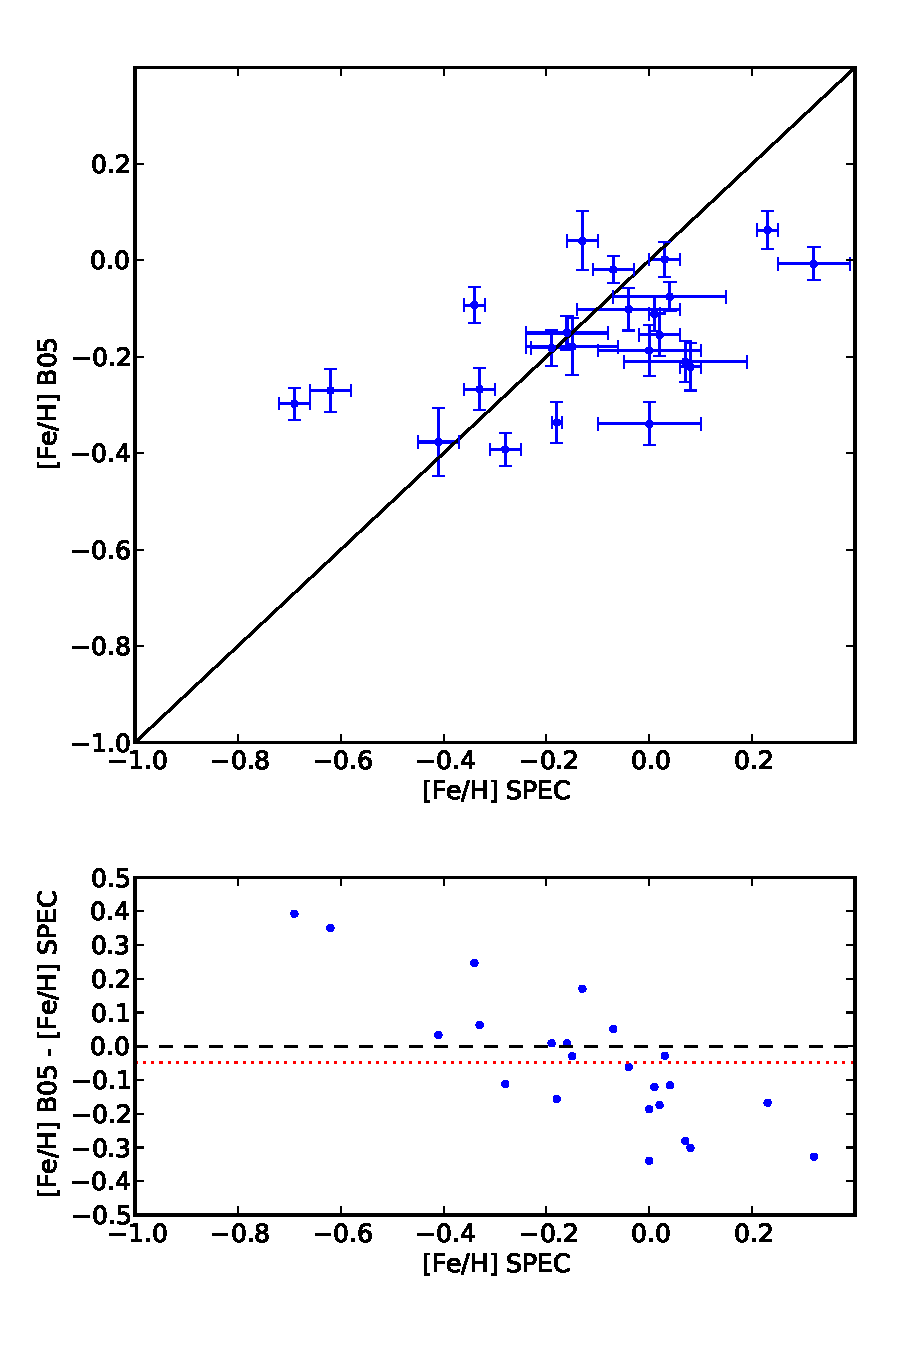
\includegraphics[scale=0.35]{pics/fehfehb051v4.pdf}}
\subfigure[B05(2) Calibration]{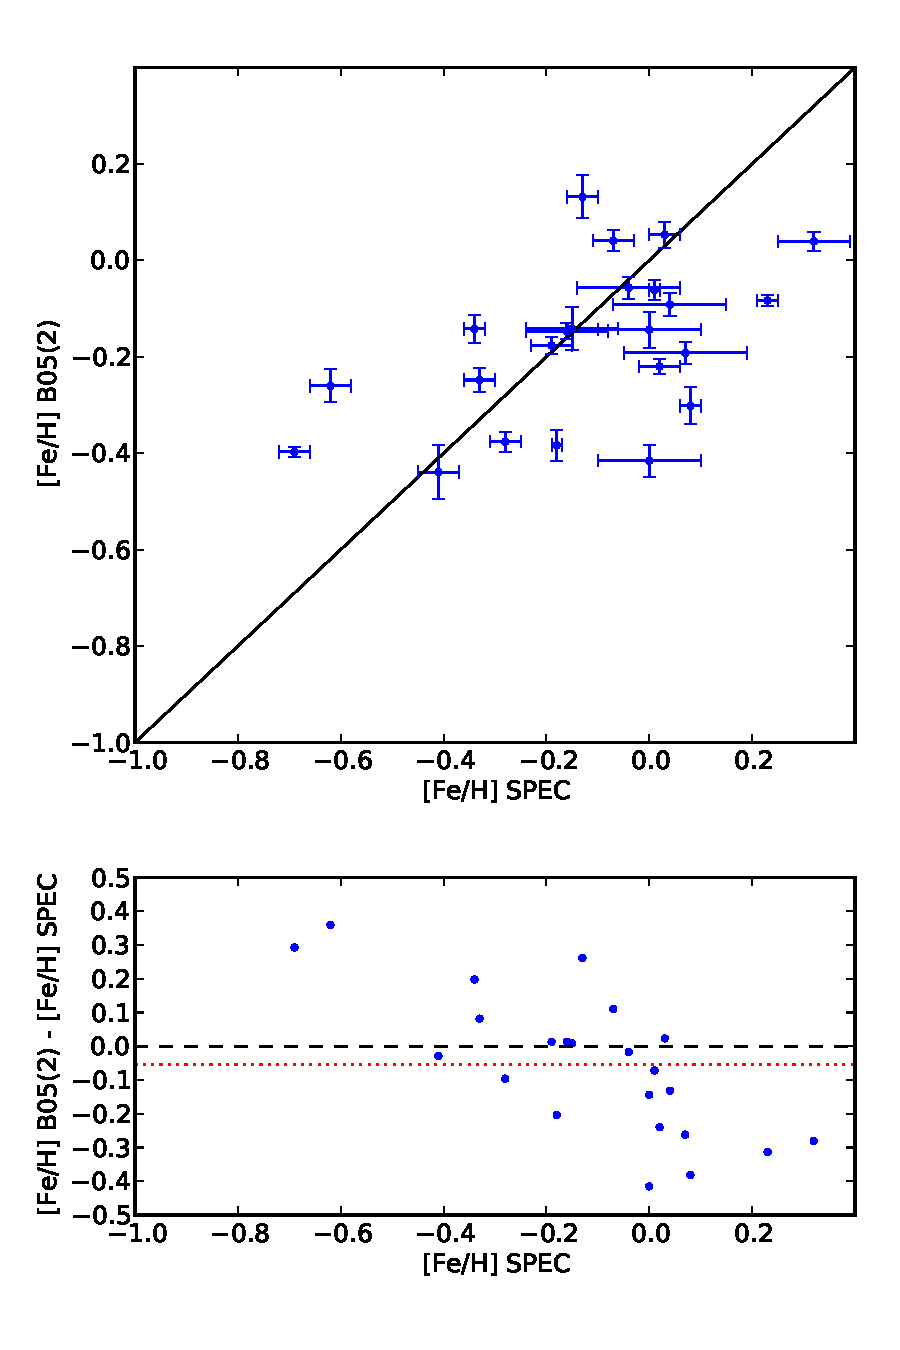
\includegraphics[scale=0.35]{pics/fehfehb052v4.pdf}}
%\subfigure[C08 Calibration]{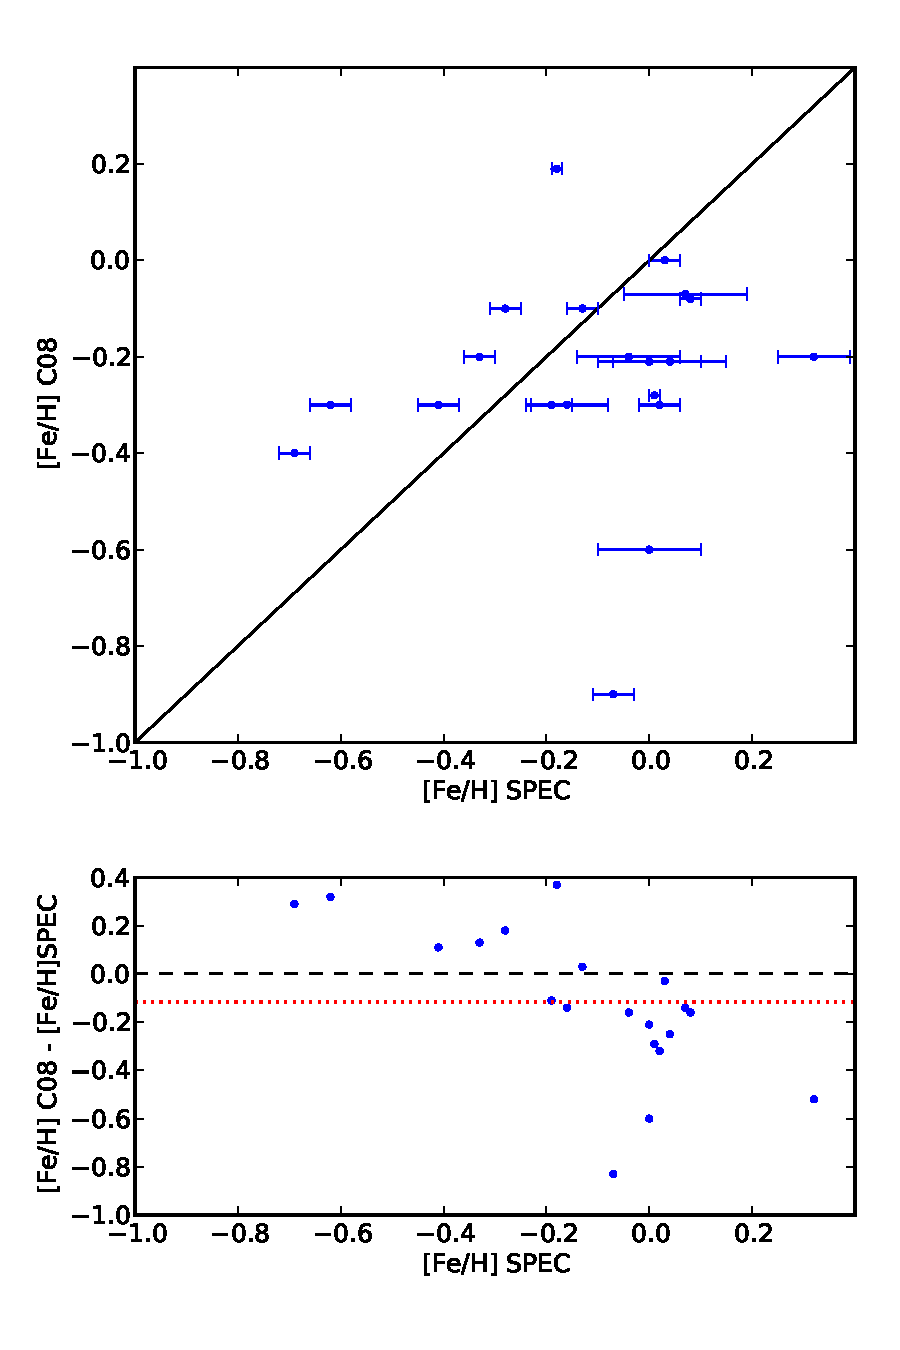
\includegraphics[scale=0.35]{pics/fehfehc08v4.pdf}}
\subfigure[JA09 Calibration]{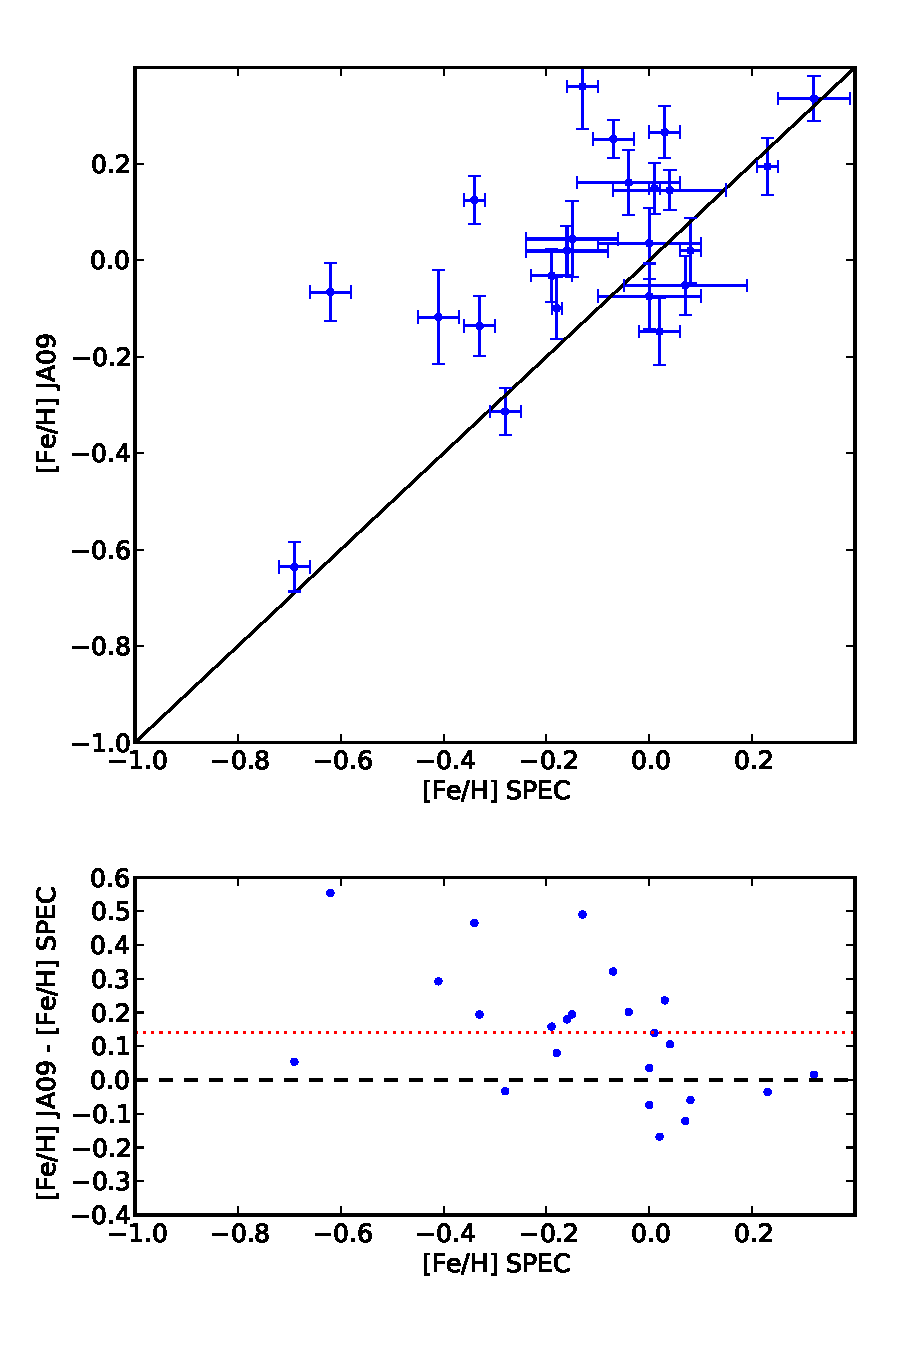
\includegraphics[scale=0.35]{pics/fehfehja09v4.pdf}}
\subfigure[SL10 Calibration]{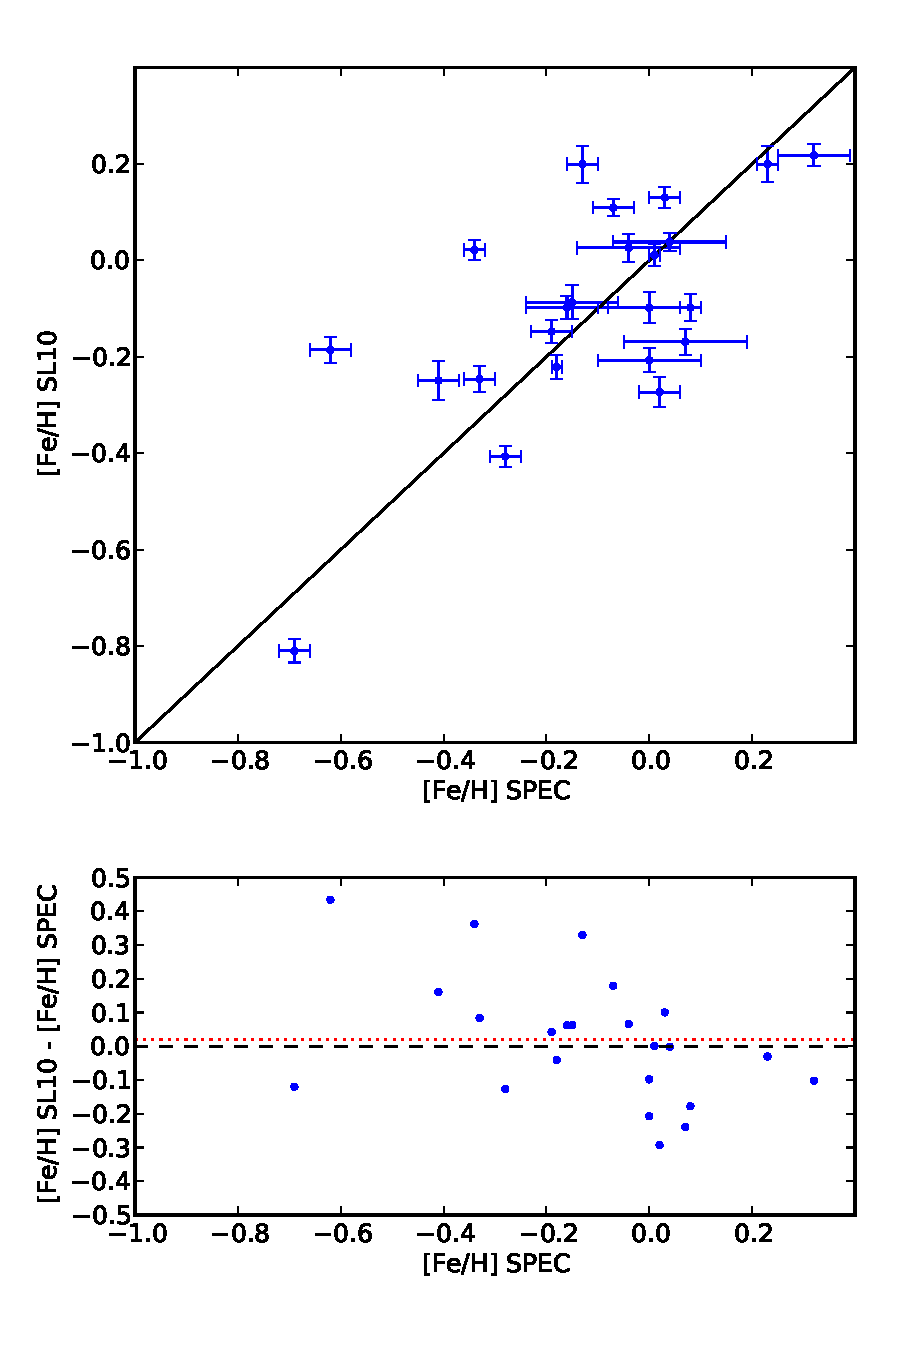
\includegraphics[scale=0.35]{pics/fehfehsl10v4.pdf}}
\subfigure[This paper]{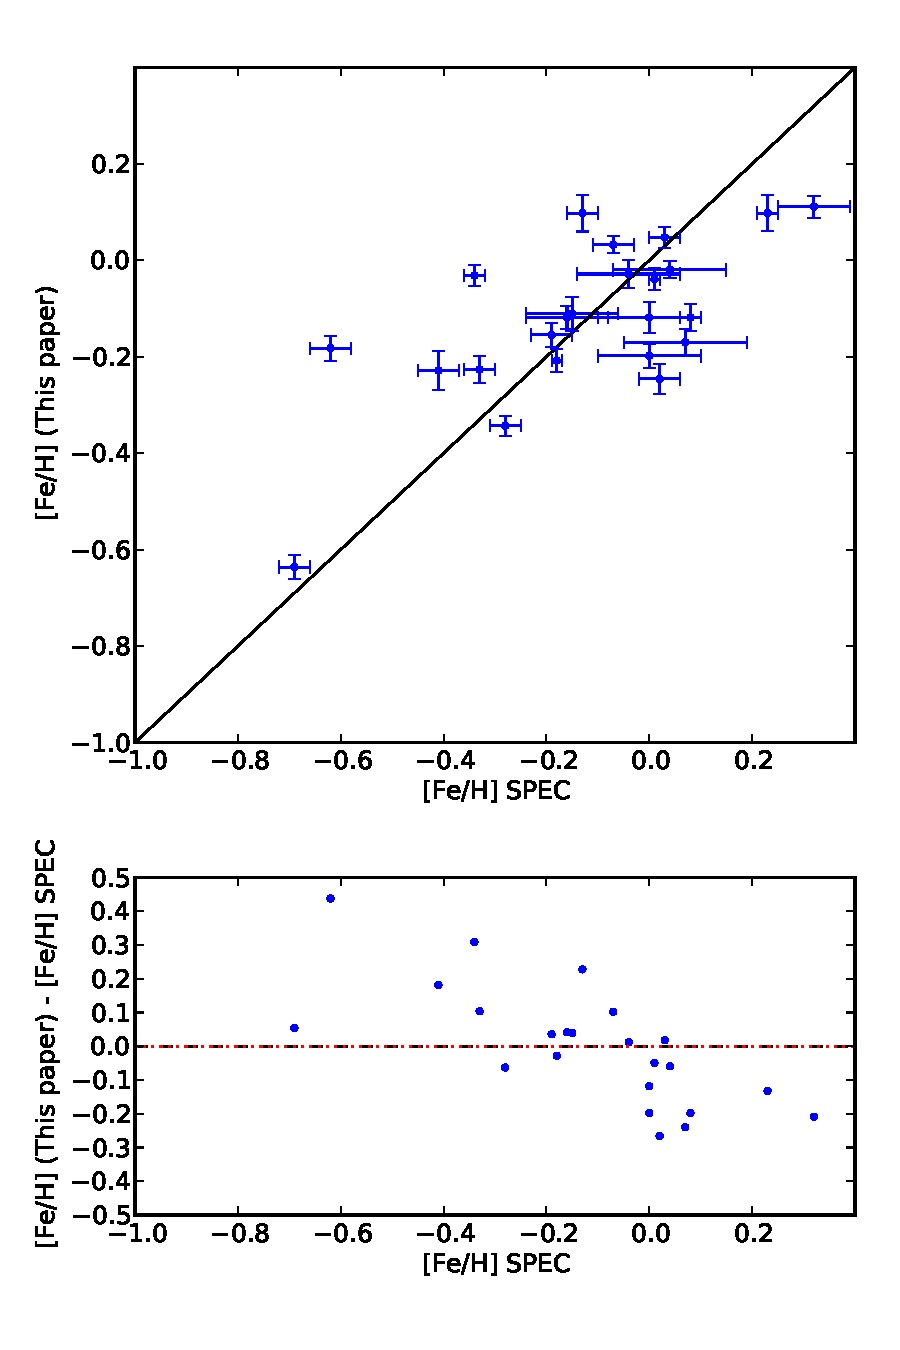
\includegraphics[scale=0.35]{pics/fehfehsl10newv4.pdf}}
\end{center}
\caption{[Fe/H] of the calibrations versus the spectroscopic metallicity. The tested calibrations are from \citet{Bonfils-2005} (a and b), \citet{Johnson-2009} (c), and \citet{Schlaufman-2010} (d). The (e) panel depicts the update we did of the calibration of \citet{Schlaufman-2010} using the sample of this paper. The blue dots with error bars represent the data points. The black line depicts a one to one relationship. The metallicity difference between the values of the calibrations and the spectroscopic measurements is shown below each [Fe/H]-[Fe/H] plot. The black dashed line is the zero point of the difference, and the red dotted line represents the average of the metallicity difference.  }
\label{fehfeh}
\end{figure*}

\begin{table*}[]
\caption{Comparison of the offset, rms, residual mean square (RMS$_{P}$), and adjusted square of the multiple correlation coefficient (R$^{2}_{ap}$) of the calibrations of \citet{Bonfils-2005}, \citet{Casagrande-2008}, \citet{Johnson-2009}, and \citet{Schlaufman-2010} applied to our data. The``This paper'' calibration is a update to the \citet{Schlaufman-2010} calibration using the sample of this paper.} %The $RMS_{P}$ and $R^{2}_{ap}$ definitions were taken from \citet{}.}
\label{stats}
\scriptsize
\begin{center}
\begin{tabular}{l r r r r}

\hline
\hline
Calibration Source + equation & offset & rms & RMS$_{P}$ & R$^{2}_{ap}$  \\
	&[dex] &[dex] & [dex] & \\ 
\hline
B05 : $[Fe/H] = 0.196 - 1.527M_{K} + 0.091M_{K}^{2} + 1.886(V-K) - 0.142(V-K)^{2}$ & $-0.05\pm0.04$ & $0.20\pm0.02$ & $0.04\pm0.01$ & $0.32\pm0.22$ \\
B05(2) : $[Fe/H] = -0.149 - 6.508\Delta M, \Delta M = Mass_{V} - Mass_{K}$ & $-0.05\pm0.04$ & $0.21\pm0.02$ & $0.05\pm0.01$ & $0.22\pm0.34$ \\
%C08 : - & -0.12 & 0.05 & 0.32 & 0.04 & 0.11 & 0.02 & -0.53 & 0.47 \\
JA09 : $[Fe/H] = 0.56\Delta M_{K} - 0.05, \Delta M_{K} = MS - M_{K}$ & $0.14\pm0.04$ & $0.24\pm0.04$ & $0.06\pm0.02$ & $0.06\pm0.49$ \\
SL10 : $[Fe/H] = 0.79\Delta (V-K) - 0.17, \Delta (V-K) = (V-K)_{obs} - (V-K)_{fit}$ & $0.02\pm0.04$ & $0.19\pm0.03$ & $0.03\pm0.01$ & $0.42\pm0.28$ \\
This paper : $[Fe/H] = 0.595\Delta (V-K) - 0.158$ & $0.00\pm0.04$ & $0.17\pm0.03$ & $0.03\pm0.01$ & $0.44\pm0.23$ \\
\hline
\end{tabular}
\end{center}
\end{table*}%

\begin{table*}[]
\caption{Metallicity values from spectroscopy and for the calibrations of \citet{Bonfils-2005}, \citet{Casagrande-2008}, \citet{Johnson-2009}, and \citet{Schlaufman-2010}. The ``This paper'' column represents the [Fe/H] values of the new fit based on the \citet{Schlaufman-2010} calibration.}
\label{tablefehfeh}
\begin{center}
\begin{tabular}{r r r r r r r r r}

\hline
\hline

Primary & Secondary & \multicolumn{5}{c}{[Fe/H] [dex]}  \\
 & & Spectroscopic & B05 & B05(2) & JA09 & SL10 & This paper \\
\hline
Gl53.1A  & Gl53.1B  & 0.07 & -0.21 & -0.19 & -0.05 & -0.17 & -0.17 \\
Gl56.3A  & Gl56.3B  & 0.00 & -0.34 & -0.42 & -0.07 & -0.21 & -0.20 \\
Gl81.1A  & Gl81.1B  & 0.08 & -0.22 & -0.30 & 0.02 & -0.10 & -0.12 \\
Gl100A  & Gl100C  & -0.28 & -0.39 & -0.38 & -0.31 & -0.41 & -0.34 \\
Gl105A  & Gl105B  & -0.19 & -0.18 & -0.18 & -0.03 & -0.15 & -0.15 \\
Gl140.1A  & Gl140.1B  & -0.41 & -0.38 & -0.44 & -0.12 & -0.25 & -0.23 \\
Gl157A  & Gl157B  & -0.13 & 0.04 & 0.13 & 0.36 & 0.20 & 0.10 \\
Gl173.1A  & Gl173.1B  & -0.33 & -0.27 & -0.25 & -0.14 & -0.25 & -0.23 \\
Gl211  & Gl212  & 0.04 & -0.08 & -0.09 & 0.15 & 0.04 & -0.02 \\
Gl231.1A  & Gl231.1B  & 0.01 & -0.11 & -0.06 & 0.15 & 0.01 & -0.04 \\
Gl250A  & Gl250B  & -0.15 & -0.18 & -0.14 & 0.04 & -0.09 & -0.11 \\
Gl297.2A  & Gl297.2B  & 0.03 & 0.00 & 0.05 & 0.27 & 0.13 & 0.05 \\
Gl324A  & Gl324B  & 0.32 & -0.01 & 0.04 & 0.34 & 0.22 & 0.11 \\
Gl559A  & Gl551  & 0.23 & 0.06 & -0.08 & 0.19 & 0.20 & 0.10 \\
Gl611A  & Gl611B  & -0.69 & -0.30 & -0.40 & -0.64 & -0.81 & -0.64 \\
Gl653  & Gl654  & -0.62 & -0.27 & -0.26 & -0.07 & -0.19 & -0.18 \\
Gl666A  & Gl666B  & -0.34 & -0.09 & -0.14 & 0.12 & 0.02 & -0.03 \\
Gl783.2A  & Gl783.2B  & -0.16 & -0.15 & -0.15 & 0.02 & -0.10 & -0.12 \\
Gl797A  & Gl797B  & -0.07 & -0.02 & 0.04 & 0.25 & 0.11 & 0.03 \\
GJ3091A  & GJ3092B  & 0.02 & -0.15 & -0.22 & -0.15 & -0.27 & -0.25 \\
GJ3194A  & GJ3195B  & 0.00 & -0.19 & -0.14 & 0.04 & -0.10 & -0.12 \\
GJ3627A  & GJ3628B  & -0.04 & -0.10 & -0.06 & 0.16 & 0.03 & -0.03 \\
NLTT34353  & NLTT34357  & -0.18 & -0.34 & -0.38 & -0.10 & -0.22 & -0.21 \\


\hline
\end {tabular}
\end{center}
\end{table*}


\section{The latest metallicity measurements and calibrations}
\label{latest}



%Here, we're going to describe in detail the photometric calibrations of \citet{Bonfils-2005} (hereafter B05(1) for the \{$(V-K) - M_{K}$\} calibration, and B05(2) for the mass calibration), \citet{Johnson-2009} (hereafter JA09) and \citet{Schlaufman-2010} (hereafter SL10). A discussion of the results will take place in section \ref{discussion}. %The \citet{Casagrande-2008} (hereafter C08) and \citet{Rojas-Ayala-2010} calibrations are described in the Appendix. 


%The calibration tests consist in the comparison between the metallicities obtained from the FGK companions of the M dwarfs and the results from each of the metallicity calibrations, namely, the two \citet{Bonfils-2005} calibrations (hereafter B05(1) for the V-K, M$_{K}$ calibration, and B05(2) for the mass calibration), the \citet{Casagrande-2008} (hereafter C08), the \citet{Johnson-2009} (hereafter JA09), and \citet{Schlaufman-2010} (hereafter SL10) calibrations. The values of the calibrations were calculated from their respective expressions (see Table \ref{stats}) except in the case of the \citet{Casagrande-2008} calibration, where no expression is available: the metallicity values were kindly provided by Luca Casagrande, using the VRIJHK$_{S}$ photometry from this paper.

\subsection{Calibration of \citet{Bonfils-2005}}

\citet{Woolf-2005} measured equivalent widths of atomic lines from high resolution spectra of 35 M and K dwarfs, as classically done for FGK dwarfs, but with updated atmospheric models. Faced by models' limitations, they apply this approach on the M dwarfs with the earliest ($T_{eff} > 3500$ K) and most metal-poor (median [Fe/H]$ = -0.89$ dex) subtypes. They later extended the study to 32 additional stars \citep{Woolf-2006}, and show that metallicity correlates with CaH and TiO molecular indices, without proposing a calibration though. %{\it This calibration has an uncertainty of $\pm$0.30 dex.} {\bf I don't like that last statement : the goal of the paper is to test the calibrations; we should distinguish better the precision reported by the authors from the precision evaluated by our paper.} {\bf Beside, is it possible to test this calibration with our sample ?}

If the molecular bands render model-based techniques difficult, they have photometric effects that are nevertheless useful to retrieve the metallicity. Increased abundances in TiO and VO shift a large amount of flux from the visible (dominated by the opacities of these species) to the infrared (where the flux is re-radiated). For a given mass, the bolometric luminosity is concurrently diminished when the metallicity increases. Both effects work together in the visible and largely cancel in the infrared, such that {\color{green}(at least in the [Fe/H] and T$_{eff}$ range of this study)} the V magnitude is largely dependent on metallicity while infrared magnitudes are not \citep{Chabrier-2000, Delfosse-2000}.

B05 used that effect as a metallicity scale, and to calibrate that scale, used binary (or multiple) stars with a FGK primary and a M dwarf secondary. The calibration is based on a $\{(V-K)-M_K\}$ color-magnitude diagram. The metallicity was measured on the primaries with a classical line-by-line analysis and assumed to be the same for the M-dwarf components. To make a larger sample, they pool their metallicity measurement with \citet{Woolf-2005}'s determination and derived a calibration with a $\sim$0.2 dex dispersion.
%The second one takes advantage of the linear relationship between metallicity and the difference between masses calculated from the V- and K-band Mass-Luminosity relations of \citet{Delfosse-2000}.
%\textbf{An alternative approach, introduced by \citet{Bonfils-2005}, is based on the measurement of metallicities from FGK high-resolution spectra in binary or multiple systems where one of the lesser bright stars is an M dwarf. The metallicity of the latter is inferred from the former. Then, a photometric metallicity calibration is established, based on the fact that the V photometry correlates with [Fe/H] whereas the K photometry does not. The metallicity effect of the V band was first suggested by \citet{Delfosse-2000}, and then confirmed by \citet{Bonfils-2005}. \citet{Johnson-2009}, and \citet{Schlaufman-2010} also used a similar technique to create metallicity calibrations for M dwarfs. All calibrations depend on precise parallaxes from the Hipparcos sattelite \citep{Perryman-1997}, and this does mean that these studies are limited to stars in the solar neighbourhood. }
Then, they used the calibration to measure the metallicity distribution of a volume-limited sample of 47 M dwarfs and found them slightly metal poor compared to FGK stars (by 0.07 dex\footnote{Mistakenly quoted to be a 0.09 dex difference in \citet{Johnson-2009}}), with a modest significance of 1.3~$\sigma$. After few more planets have been detected, and as already mentioned above, \citet{Bonfils-2007} used the same calibration to compare M dwarfs with and without planets and found that planet hosts are marginally metal rich.


%\sout{B05 found that the mean metallicity of M dwarfs with planets is $-$0.11 dex, which contrast sharply with the value found for FGK stars ($+$0.15 dex). Moreover, they found a hint that the metallicity of M dwarfs, using the calibration, in their complete, volume limited sample of FGKM dwarfs may have a $\sim 0.07$ dex shift toward lower metallicities, when compared to the full sample. This may imply that the decreased frequency of Jovians around M dwarfs is a reflection of their lower metallicities rather than their lower masses.}% However, this difference is not statistically distinguishable from their full sample. \citet{Bonfils-2005} calibration has an uncertainty around $\pm$0.20 dex.

B05 and \citet{Bonfils-2006} also examined the metallicity distribution of M dwarfs, without distinguishing planet hosts from single stars, and compared the distribution with FGK stars. Applying their calibration to a volume limited sample of 47 M dwarfs and comparing to 1,000 FGK stars from the CORALIE planet-search program, they found M dwarfs to be slightly metal poor by 0.07 dex, albeit with a confidence level of 2.6~$\sigma$ only.

With this paper's sample, we measure that the B05 calibration has an offset of $-0.05\pm0.04$ dex and a dispersion of 0.20$\pm$0.02 dex. Interestingly, correcting from that offset almost cancels the metallicity difference between M dwarfs and FGK stars. Naturally, it does not affect the possible metallicity difference between M dwarfs with and without known planets. The negative offset is in line with the result of SL10 (see Section \ref{Schlaufman}) that B05 underestimates, in general, the true value of [Fe/H].

%{\color{green} SL10 reports that the B05 calibration has a R$^{2}_{ap}$ value lower than 0.05. We find, however, that the R$^{2}_{ap}$ value for the B05 model is higher than 0.05 ($0.32\pm0.22$) despite having large uncertainties. Therefore, the statement of SL10 that their model explains almost an order of magnitude more of the variance of the calibration sample, relative to the B05 model, is not confirmed. The discrepancy between the results may result from using different $p$  values in Eq. (\ref{rmsp}), as this may induce large changes in R$^{2}_{ap}$ . We used $p=0$ in Eq. (\ref{rmsp}) for all calibrations (except in the case of our new calibration), whereas SL10 might have used other values.}

SL10 reports a $R^{2}_{ap}$ value lower than 0.05 for the B05 calibration and stated that their model explains almost an order of magnitude more of the variance of the calibration sample. In Sect. 3, we noted, however, that the value of p is uncertain when there is an overlap between samples. Moreover, we compute large uncertainties for $R^2_{ap}$ and point it is probably not a robust estimator. Against our sample, and using p=0, we find $R^{2}_{ap}=0.32\pm0.16$ dex. That value is higher than reported by SL10 and tends, therefore,  to mitigate the improvement from this calibration.{\color{blue}{Is this remark in the last phrase too strong? What is your opinion?}}

%\sout{The B05(2) calibration has similar results but with a marginally bigger dispersion ($-0.05\pm0.03$ dex and $0.21\pm0.02$ dex respectively).

In addition to the commonly used calibration, B05 also provides another expression to evaluate [Fe/H]. That second expression, labeled B05(2) in Table \ref{stats}, is based on the difference between the V- and K-band expressions of the mass-luminosity relation given in \citet{Delfosse-2000}. Against this paper sample, both expressions given in B05 perform equally, with B05(2) having a marginally higher dispersion. In the remaining of this paper we therefore elude B05(2).

%The RMS_{p} value is 0.04 dex, similar to the lowest value of 0.03 dex of \citet{Schlaufman-2010} calibration. 
 

\subsection{Calibration of \citet{Johnson-2009}}

Since our first attempt, further works have been proposed to improve on the metallicity calibration. Notably, \citet{Johnson-2009} have argued that M dwarfs should have the same metallicity as FGK stars and chose accordingly to fix their mean metallicity to the solar-neighborhood value ($-0.05$ dex). From a volume-limited sample of FGK dwarfs from the SPOCS sample \citep{Valenti-2005}, they next determined a sequence representative of the average M dwarf in the $\{(V-K)-M_K\}$ color-magnitude diagram proposed by \citet{Bonfils-2005}. Then, they modeled the metallicity as the linear distance to that main sequence along $M_{K}$. To calibrate that scale, they used the metallicity of 6 metal-rich M dwarfs with values known from FGK primary components.

Fixing the metallicity of M dwarfs is a strong assumption that JA09 have motivated with two lines of arguments. Firstly, they presented [Fe/H] measurements for 109 G0-K2 stars that span effective temperatures from 4900 to 5900 K. They measured a weak Pearson correlation coefficient and concluded that, because no metallicity gradient is seen for this temperature range, no metallicity difference is to be expected for the cooler M dwarfs. We note, however, that when we did a linear fit to this data set ([Fe/H] = $9.74\times10^{-5} . (T_{\rm eff}-5777)  - 0.04$) we found that any extrapolation to the cooler M dwarfs (2700$<$Teff$<$3750, from M7 to M0 spectral type) actually allows for a wide range of metallicities ($-0.32 < $ [Fe/H] $ <  - 0.22$), that are values even lower than the [Fe/H] difference seen in B05. Secondly, they measured a large (0.32 dex) difference between B05 calibration and the primary-measured values for the 6 chosen metal-rich M dwarfs. This robustly points for a systematic offset in B05 calibration, at least for the metal-rich part, but did not anchor the mean metallicity of M dwarfs. 

In the high-metallicity range, where JA09 calibrators were chosen, the calibration matches well the metallicities of our sample. With decreasing metallicity JA09 calibration however gives too metal rich values (as already pointed out by SL10, see below). %Table \ref{stats} and Fig.~\ref{fehfeh} report our tests . 
Notably, we measure a global offset of $+0.14\pm0.04$ dex and a dispersion of $0.23\pm0.04$.
%\sout{In our paper, we can see from Fig. \ref{fehfeh} and Table \ref{stats} that the JA09 calibration suffers from a big offset ($0.14\pm0.03$), and with a dispersion of $0.23\pm0.03$. {\color{green} This means that JA09 overestimated their estimation for the metallicity. When comparing this calibration with the ones from \citet{Bonfils-2005}, we can observe that the latter ones have a lower offset, rms, $RMS_{p}$ values, and a higher $R^{2}_{ap}$ value.}}


%Their results imply that the metal rich stars of \citet{Bonfils-2005} are systematically underestimated, by an average of 0.32 dex, suggesting that this might be due to a lack of metal rich stars in their sample or due to the use of poor V magnitudes. {\color{blue} This paragraph need to be re-phrased.}

%They conclude that M dwarf planet hosts follow the same trend as FGK stars, that is, they are preferentially metal rich. They also suggest that the lack of Jovian planets around M dwarfs is mostly correlated to a lower stellar mass and not to a lower value of [Fe/H], being more consistent with the works of planetary formation around M stars (i.e. \citeauthor{Laughlin-2004} \citeyear{Laughlin-2004}; \citeauthor{Ida-2005} \citeyear{Ida-2005}).

\subsection{Calibration of \citet{Schlaufman-2010}}
\label{Schlaufman}
Following on B05 and JA09 works, \citet{Schlaufman-2010} improved on our comprehension of M dwarf metallicity and its calibration.

First, they have shown that, for M dwarfs and FGK stars to share the same mean metallicity, a kinematic match is equally important as a volume-limited match for both samples. Indeed, the different kinematic populations of our Galaxy have significant different mean metallicities and the mean metallicity of small samples could fluctuate with the number of stars from each population. To overcome this statistical noise, they draw a volume-limited sample of F and G stars from the Geneva-Copenhagen Survey that matches kinematically the volume limited sample of M dwarfs used by JA09. They found that the sample of FGK stars has a mean metallicity of $\simeq - 0.14\pm0.06$ dex, which is $0.09$ dex lower than the value adopted by JA09. 

Second, they use \citet{Baraffe-1998} models to compute [Fe/H] isocontours. They show that in a \{(V$-$K)$-$M$_K$\} diagram, a change in [Fe/H] results essentially in a change in (V$-$K), and almost no change in M$_{K}$. The [Fe/H] is therefore better calibrated by (V$-$K) and they propose the calibration should be based on a linear function of the (V$-$K) distance in a \{(V$-$K)$-$M$_K$\} diagram. To remain free of any assumption regarding the mean metallicity of M dwarfs, they kept the ordinate at the origin of the calibration as a free parameter.


% Not clear to me ....
%Following the work of \citet{Johnson-2009}, \citet{Schlaufman-2010} created a very similar calibration but using a volume-limited and kinematically matched sample to test if the value found for the mean M dwarf main sequence metallicity using FGK primaries (with M dwarf secondaries) were compatible with each other. A kinematically matched sample was used to screen out stars with outlier kinematics. They conclude that both samples are statistically indistinguishable.}

%vef melhor esta questao dos catalogos, falar com o Xavier sobre isto.
%, the Geneva-Copenhagen survey \citep{Nordstrom-2004}. They claim that this catalogue is more unbiased and outlier-sensitive when compared to other catalogues, having a mean MS metallicity value for the M dwarfs of -0.14 dex as opposed to -0.05 dex of \citet{Johnson-2009}. 
%Using models from \citet{Baraffe-1998}, they show that the metallicity correlates best with horizontal shifts in the $V-K_{s}$,$M_{K_{s}}$ plane. For this reason, they compute the distance from the M dwarf main sequence to the M dwarf star only in the $V-K_{s}$ direction. 

%Compared to previous calibrations, their results imply that \citet{Bonfils-2005} and \citet{Johnson-2009} have respectively underestimated and overestimated the metallicity at the extremes of their range. %\sout{They conclude that their results suggest that metal rich M dwarfs are more likely to host planets, as in FGK stars, and they claim that there is a hint that this correlation might extend to low-mass planets as well. Their result for low mass planets is in opposition to results obtained for low-mass planets orbiting FGK stars, which state that there is no significative relation between metallicity and the existence of low-mass planets (e.g. \citeauthor{Udry-2007b} \citeyear{Udry-2007b}; \citeauthor{Sousa-2008} \citeyear{Sousa-2008}).} 
%{\color{blue}I suggest to deport the discussion on the planet-metallicity correlation to the conclusion. Also, we should not only report the claims but be critical and objective.} 
 

We used the SL10 sample to measure its dispersion and obtained a value of $0.14\pm0.02$ dex. But against our test sample, we measure a higher value of $0.19\pm0.03$. The dispersion difference may be explained by a larger dispersion, in our sample, of the $M_{k}$ vs $(V-K)$ relationship, that translates solely into a larger range of the metallicity, as the effective temperature range is approximately the same. To test this hypothesis we measured the dispersion of a sub-sample of 18 stars inside the metallicity range of the sample of SL10. We obtained a dispersion value of $0.15\pm0.02$ dex, very similar to the result obtained for the SL10 sample. This may mean that the dispersion of our sample has physical roots rather that being due to measurement uncertainties.  

We also measure an offset of $0.02\pm0.04$ dex. Both offset and rms improved over B05 and JA10 calibrations.


%The SL10 and the B05 calibrations have a similar value of rms and RMS$_{p}$, though the values of SL10 are marginally lower. Regarding the offset and the R$^{2}_{ap}$ values, the SL10 calibration has lower values (0.02 dex and 0.42 respectively) than the ones from the B05 calibration (-0.05 dex and 0.32 respectively). This suggests that the calibration that is best suited for the prediction of the metallicity is the one of SL10 and that this model is the best suited for explaining the variance of the data. 

%The results also show that the B05 and JA09 models respectively underestimate and overestimate the metallicity in general, as it is clearly seen in Fig. \ref{fehfeh} in accordance with the previous findings of SL10. {\color{blue} ??? I don't see it ! Or maybe you are talking about something that is not related to the comparison of SL10 calibration and this paper's sample. And then it has to be in a different paragraph...} 

\subsection{Updating the \citet{Schlaufman-2010} calibration}

%{\color{blue} Here, say that, with our new sample, we update the metallicity calibration following Schlaufman \& Laughlin prescription. Give the expression of the new calibration and its dispersion.}

We have established a new fit following the SL10 prescription, using the $RMS_{p}$ free parameter $p = 2$ (see Section \ref{test}). The expression for the new metallicity calibration is 

\begin{eqnarray}
[Fe/H] = 0.57 \Delta (V-K_{s}) - 0.17, \\
\indent \Delta(V-K_{s}) = (V-K_{s})_{obs}-(V-K_{s})_{iso}, \nonumber
\label {sl10new}
\end{eqnarray}
%\S
where $(V-K_{s})_{obs}$ is the observed photometric difference between V- and $K_{s}$-band and $(V-K_{s})_{iso}$ is a 5th order polinomial as a function of $M_{K_{s}}$ that denotes the mean main sequence of the Solar neighborhood from the SPOCS catalog. This expression was taken from \citet{Schlaufman-2010} and was defined originally as $M_{k}$ as a function of $(V-K_{s})$ by \citet{Johnson-2009}. \sout{It has the following coefficients in increasing order: $51.1413, -39.3756, 12.2862, - 1.83916, 0.134266,$ and $-0.00382023$.} 

From the results shown in Table \ref{stats}, we can observe that there are no significant differences between this new fit and the original calibration. The rms of the new fit is tighter just by 0.02 dex (from $0.19\pm0.03$ to $0.17\pm0.03$ dex), and the offset is now $0.00\pm0.04$, as expected. The R$^{2}_{ap}$ value are similar ($0.42\pm0.28$ vs $0.44\pm0.23$) despite having big uncertainties, and the $RMS_{p}$ value is the same as the SL10 calibration. This means that the calibration of SL10 is still valid using our new data.

The dispersion of the sample, seen in all the plots of Fig. \ref{fehfeh} is much higher than the uncertainties of the measurements. This means that we are not limited by measurement uncertainties. If this was not the case the points would be much closer to the identity line.

We must note the possible existence of a trend with spectroscopic [Fe/H], having a negative slope, for the B05, B05(2), and the calibration presented in this paper. This may also be the case for the remaining calibrations, if we ignore the data point with the lowest value of [Fe/H]. The B05 and B05(2) calibrations also seem to overestimate the metallicity for spectroscopic [Fe/H] $< -0.4$. Regarding higher metallicities, above 0.2 dex, only the calibrations of JA09 and SL10 seem to accurately predict the spectroscopic metallicities: all the other calibrations underestimate the [Fe/H] value. We do not know the cause of the [Fe/H] trend, but this may mean that the current models are missing a higher order trend.


%{\color{green} Nonetheless, we decided to correct this trend from our calibration. First, we calculated the slope and offset by doing a linear fit. Then, we subtracted this value and corrected the slope, as seen in Fig. \ref{rescor}. The corrected [Fe/H] calibration is now: 
%
%\begin{eqnarray}
%[Fe/H] &=&0 .57 \Delta (V-K_{s}) - 0.17 - \Delta [Fe/H], \\
%\Delta [Fe/H] &=& a.[Fe/H]+b, \nonumber 
%\label {sl10cor}
%\end{eqnarray}
%
%where $a = -0.5434$ and $b = -0.0673$.}


\begin{figure}[h]
\begin{center}
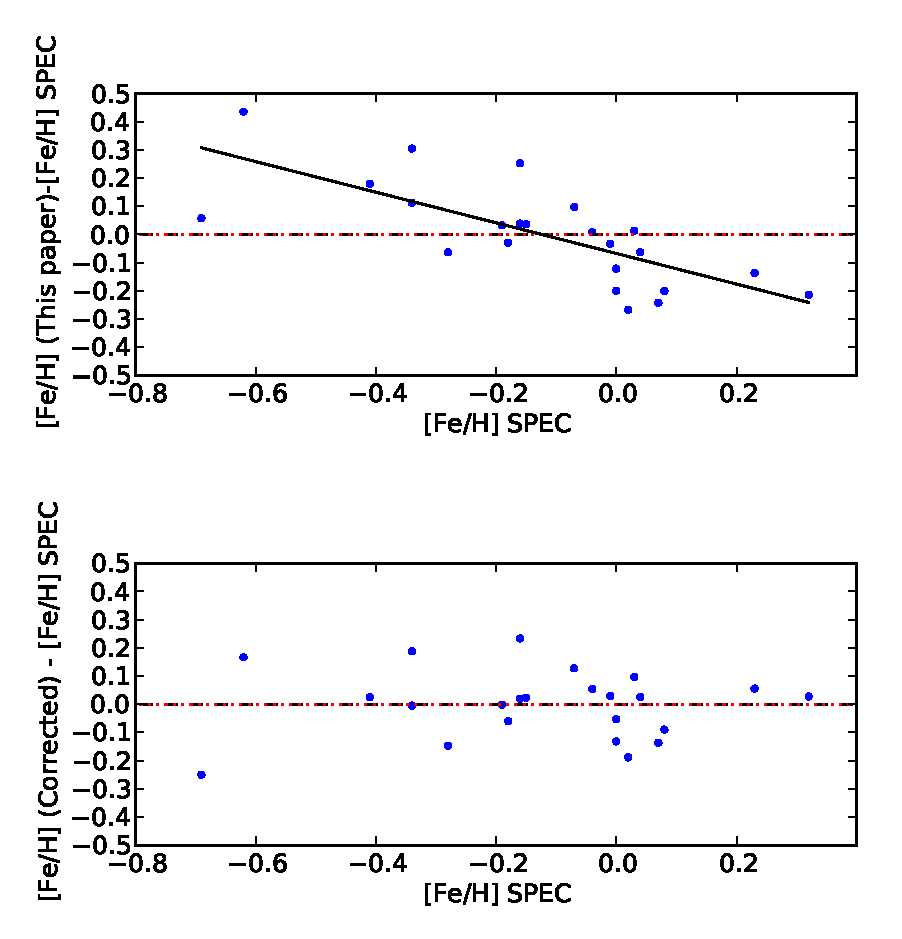
\includegraphics[scale=0.5]{pics/residual_cor.pdf}
\end{center}
\caption{Correction of the trend of the [Fe/H] calibration of this paper. Top: residuals without the correction. The black line is the linear fit to the trend; Bottom: residuals after the correction.}
\label{rescor}
\end{figure}



%\subsection{Divers things to be changed (or removed)}

%{\bf \color{blue}I suggest the paper focuses on photometric calibrations only, which implies not talking about Valenti/Bean approaches, defering the comparison with Casagrande's technique to an appendix, and discussing Rojas et al.'s work in the discussion part only.}
% {The high-resolution spectral synthesis is starting to produce its first results for M dwarfs (e.g. \citeauthor{Valenti-1998} \citeyear{Valenti-1998}, \citeauthor{Bean-2006} \citeyear{Bean-2006}). However, the technique does not yet reproduce all the fine details of a high-resolution spectra, due to a lack of the proper opacities and molecular transitions for the used model atmospheres. \citet{Bean-2006} used this technique to determine precise stellar parameters of M dwarfs. He found that the uncertainties regarding the determination of metallicity were around 0.12 dex. However, this value does not take into account systematic errors or errors that may come from the models.} %Therefore, the results of this work should be taken with care.

%A completely different technique was devised by \citet{Casagrande-2008} based on his previous study of FGK stars using the infrared flux method \citep{Casagrande-2006}. In order to adapt this method to M dwarfs, optical bands were added, creating the so-called MOITE, Multiple Optical and Infrared TEchnique.  The calculated metallicities have a very good agreement with \citet{Bonfils-2005} results. The internal uncertainties are reported as $\sim$ 0.2 dex and the total uncertainty is estimated to be between 0.2 and 0.3 dex.

%FAZER UMA PEQUENA REFERENCIA AO BEAN (2006). DONE





%A classical spectroscopic analysis gets more difficult with the increase of the spectral subtype, as the number of several diatomic and triatomic molecules. 

%During the last few years there have been several attempts at creating a metallicity calibration for M dwarfs. Establishing such calibration is important 







%\section{The test}
%\label{test}
%
%\begin{table*}[]
%\caption{Boostrap analysis of the data. 10.000 trials were made, where each trial used a random set of data comprised by 1 $\sigma$ of the full sample. The table depicts the standard deviation of the evaluated parameters (offset, rms, RMS$_{p}$, and R$^{2}_{ap}$), for all calibrations.}
%\label{bootstrap}
%\begin{center}
%\begin{tabular}{l c c c c}
%
%\hline
%\hline
%Calibration  & $\sigma$ offset & $\sigma$ rms  & $\sigma$ RMS$_{p}$  & $\sigma$ R$^{2}_{ap}$ \\
%\hline
%B05(1) & 0.03 & 0.02 & 0.01 & 0.16 \\
%B05(2) & 0.03 & 0.02 & 0.01 & 0.26 \\
%C08 & 0.05 & 0.04 & 0.02 & 0.56 \\
%JA09 & 0.03 & 0.03 & 0.01 & 0.31 \\
%SL10 & 0.03 & 0.02 & 0.01 & 0.18 \\
%SL10(NEW) & 0.02 & 0.02 & 0.01 & 0.15 \\
%\hline
%\end {tabular}
%\end{center}
%\end{table*}


%{\color{blue} Now, a large fraction of that section is given in Sect. 3 and 4. Not all the information written below has been reported above. In particular, the results of the test for each calibration. Please, Vasco, can you report the result of the test in the respective sub-sections of each calibration (\S4.1, 4.2, ...) ?}

%The calibration tests consist in the comparison between the metallicities obtained from the FGK companions of the M dwarfs and the results from each of the metallicity calibrations, namely, the two \citet{Bonfils-2005} calibrations (hereafter B05(1) for the V-K, M$_{K}$ calibration, and B05(2) for the mass calibration), the \citet{Casagrande-2008} (hereafter C08), the \citet{Johnson-2009} (hereafter JA09), and \citet{Schlaufman-2010} (hereafter SL10) calibrations. The values of the calibrations were calculated from their respective expressions (see Table \ref{stats}) except in the case of the \citet{Casagrande-2008} calibration, where no expression is available: the metallicity values were kindly provided by Luca Casagrande, using the VRIJHK$_{S}$ photometry from this paper.
%
%We also decided to do a refit of the SL10 expression with our sample in order to verify, search for systematics, and possibly optimize the original one. The new model is hereafter named SL10(NEW). We only did this refitting for the SL10 calibration because it is considered the best model, which is also confirmed to be the case in this paper.
%
%In order to access the quality of each calibration we calculated the following values: the offset, rms, RMS$_{p}$ and R$^{2}_{ap}$. The RMS$_{p}$ is the residual mean square and the  
%R$^{2}_{ap}$ is the adjusted square of the multiple correlation coefficient, as described by \citet{Hocking-1976} and used in the SL10 paper. The $RMS_{p}$ is defined as
%
%\begin{equation}
%RMS_{p} = \frac{SSE_{p}}{n-p}, \\
%SSE_{p} = \sum{(y_{i,model}-y_{i})^{2}},
%\label {rmsp}
%\end{equation}
%
%where $SSE_{p}$ is the residual sum of squares for a p-term model, n is the number of data points, and p is the number of free parameters. The R$^{2}_{ap}$ is defined as 
%
%\begin{equation}
%R^{2}_{ap} = 1-(n-1)\frac{RMS_{p}}{SST}, \\
%SST = \sum{(yi-\bar{y})^{2}}.
%\label {r2ap}
%\end{equation}



%A lower value of RMS$_{p}$ means that the model being tested is best suited for prediction, while a R$^{2}_{ap}$ closer to 1 signifies that the tested model explains most of the variance of the data. The values for these parameters are shown in Table \ref{stats}. We must note that we used $p = 0$ for all calibrations (except for SL10(NEW)) because we are not fitting the data but just using the values of the parameters of the original calibrations. In the case of the new fit to the SL10 calibration, we used $p=2$. 



%To test the robustness of these values, we did a bootstrap analysis where 10.000 trials were made using, for each trial, 68\% (1 $\sigma$) of randomly chosen data points from the full sample. Then, we calculated the average of the quantities described in the first test. The results for this test are described in Table \ref{bootstrap}.  





%Fig. \ref{fehfeh} shows the plots of the [Fe/H] obtained from the calibrations versus the spectroscopic [Fe/H]. The blue dots with error bars represent the data points and the black line depicts a one to one relationship. Below each plot is shown the metallicity difference between the calibrations and the spectroscopic values. The black dashed line is the zero point of the metallicity difference, and the red dotted line represents the average of the metallicity difference. Table \ref{tablefehfeh} displays the metallicity values from spectroscopy and the different calibrations, where the individual values for each star can be directly compared.


%Figs. \ref{calib} and \ref{fehfeh} show the plots of the different metallicity calibrations and the plots of the [Fe/H] obtained from the calibrations versus the spectroscopic [Fe/H], respectively. The blue dots with error bars represent the data points and the black line depicts the different calibration models and the metallicity one to one relationship, respectively. Table \ref{tablefehfeh} displays the metallicity values from spectroscopy and the different calibrations. %Table \ref{stats} displays the different equations for each calibration, \textit{when relevant}, as well as the dispersion around the mean value ($rms$), the residual mean square ($RMS_{p}$), and the adjusted square of the multiple correlation coefficient ($R^{2}_{ap}$).  $RMS_{p}$ and $R^{2}_{ap}$ were taken from \citet{Schlaufman-2010}. 






 %Nevertheless, the SL10 model has the highest R$^{2}_{ap}$ value (0.27) with the lowest dispersion (0.20). 
%The bootstrap analysis confirms that the SL10 is best calibration so far for predicting metallicities of M dwarfs.



%\textbf{We must note, however, that all calibrations seem to overestimate the metallicity for spectroscopic [Fe/H] $< -0.4$. Unfortunately, we only have one star in this region, but there is a hint that there may be a trend with a negative slope as a function of the spectroscopic metallicity in all the lower panels of Fig. \ref{fehfeh}. We do not know the cause for this trend. Regarding higher metallicities, above 0.2 dex, only the calibrations of JA09 and SL10 seem to accurately predict the spectroscopic metallicities: all the other calibrations underestimate the [Fe/H] value. }




%Regarding the remaining calibrations, the best one is the one from Sl10, which has a very small offset (-0.02 dex) and the smallest $rms$ value (0.19 dex) of all calibrations. The calibration of SL10 has the smallest value of $RMSp$ and $R^{2}_{ap}$. This means that this model is best suited for prediction as well as the best in explaining the variance of the data. This trends can be seen more clearly in Figs. \ref{residuals} and \ref{fehfeh}.







%%%METER AQUI UM PARAGRAFO SOBRE O SL10 E O NORDSTROM!

%%% O que dizer sobre a ROJAS?





\section {Summary}
\label{discussion}

%Following the plots from Fig. \ref{fehfeh} and Table \ref{stats} we can observe that all calibrations fit the data reasonably, except in the case of JA09. This calibration suffer from a big offset (0.14 dex). 


%Regarding our new fit of the SL10 calibration, we can observe that it is very similar to the original one, although a little bit tighter, with a slightly lower rms. The R$^{2}_{ap}$ value can be considered equal (0.42 vs 0.44). 

%We must remind that, in the case of this new calibration, we used $p=2$ in Eq. (\ref{rmsp}).

We have assembled a sample of M dwarf companions to hotter FGK
stars, where the system has an accurate parallax and the M~dwarf
component has accurate V and K-band photometry. Using the metallicities
of the primaries, newly measured or retrieved from the literature, 
and the assumption that the two components have identical initial 
compositions, we compared the dispersions of the \citet{Bonfils-2005}, 
\citet{Johnson-2009}, and \citet{Schlaufman-2010} photometric 
metallicity calibrations. We find that the \citet{Schlaufman-2010} 
scale, which is intermediate between \citet{Bonfils-2005} and
\citet{Johnson-2009}, has the lowest dispersion. We slightly
refine that relation, by readjusting its coefficients on our 
sample. 

We find that our tight selection of binaries with accurate 
parallaxes and photometry sample has insignficantly reduced 
the dispersion of the measurements around the calibration 
compared to looser criteria. This suggests that the dispersion, 
and therefore the random errors of the calibration, is not
defined by measurement uncertainties but rather reflects 
intrisic astrophysical dispersion.
{\em Here we should probably speculate on the possible 
underlying parameter(s). Age is unlikely: M dwarfs don't evolve away from
the main sequence within a Hubble time, and young M dwarfs that
haven't yet reached the main sequence are too few to contribute
more than occasional outliers. Rotation is one possibility. Our
assumption of identical metallicities for the two components could
perhaps break down in detail. Any other idea?}
Unless, or until, we develop a quantitative understanding of
this astrophysical dispersion, the photometric calibration 
approach may therefore have reached an intrinsic limit. 
Those calibrations also have the very practical inconvenient, 
of needing an accurate parallax. This limits their use to the 
close Solar neighborhood, at least until the GAIA catalog becomes 
available in a decade.

Alternative probes of the metallicities of M dwarfs are therefore
obviously desirable. One obvious avenue is to work from higher 
spectral resolution information, and identify spectral elements
that are most sensitive to metallicity and others which are 
most sensitive to effective temperature. We are pursuing this
approach at visible wavelengths (Neves et al. in prep.), as
do \citet[][, see Appendix 2]{Rojas-Ayala-2010} in the near 
infra-red, with encouraging results in both cases.

%, using precise metallicity determinations from binary/multiple systems and precise V(RI)$_{C}$JHK$_{S}$ photometry. {\color{green} We conclude that, at present, our updated calibration based on \citet{Schlaufman-2010} should be the one to be used to calculate the metallicities of M dwarfs} : it has the lowest zero-point offset, dispersion, RMS$_{P}$ and has the highest R$^{2}_{ap}$. %Unfortunately, we were not able to test the \citet{Rojas-Ayala-2010} calibration. Therefore, we cannot confirm or deny if this calibration is better than the one of \citet{Schlaufman-2010}. However, our limited external test with seven stars (see Appendix Section \ref{rojas}) is encouraging and suggests that this calibration should be properly tested in the future.

%\sout{We did a marginal improvement of the SL10 calibration with our sample. Despite that, we find that there are no significant differences between this new fit, the original calibration, and the older B05 calibration. The new fit is tighter by 0.02 dex (from 0.19 to 0.17 dex). We therefore conclude that the SL10 expression is valid for our sample. }



%\sout{
%The impact of the precision of V photometry on the final precision of some of the calibrations (B05, JA09, SL10) have been recently discussed. In this paper we use precise V photometry, with an average precision of $\sim$ 0.02 mag, and conclude that the use of precise photometry does not impact the final dispersion of the mentioned calibrations: there is not a significant decrease of the obtained rms when compared to the dispersion reported in the original papers. }

%\sout{The precise determination of metallicities of M dwarfs is very important in the understanding of the formation and evolution of planets around very low mass stars, as well as for studies about the star-planet connection. Some questions are left unanswered, such as which of the two parameters, [Fe/H] or mass, are the most important in the planet formation around M dwarfs, or whether the relation between the higher frequency of planets around stars that are richer in [Fe/H] is true for M stars or not. In order to answer these questions, a more precise metallicity determination is needed, either by doing a better calibration, or by exploring other approaches, such as using spectral indexes, like \citet{Woolf-2006}, and \citet{Rojas-Ayala-2010}, or by finding a way to directly measure the stellar parameters of M dwarfs, either empirically (e.g. \citeauthor{Woolf-2005} \citeyear{Woolf-2005}) or by using synthetic spectra (e.g. \citeauthor{Bean-2006} \citeyear{Bean-2006}). }
%In the near future, we aim to create a photometric metallicity calibration that can reach a precision of the order of $\sim$ 0.05 dex, as well as finding new ways to directly determine the metallicity and other parameters (such as effective temperature) from the M dwarf spectra. In this paper we did not address the planet-metallicity correlation, but we intend to do it in the future. 


%falar um pouco a dizer que infelizmente n podemos dizer grande coisa sobre os planetas mas que tentaremos responder a essas questoes num futuro proximo.
%FAZER bootstrap do sample e ESCREVER que a V photometry n e uma limitacao na determinacao do feh
%

\begin{acknowledgements}
%				      
%We thank the Swiss National Research Foundation (FNRS) and the Geneva 
%University for their continuous support to our planet search programmes. 
We would like to thank Luca Casagrande for kindly providing us the metallicities calculated from his calibration. We acknowledge the support by the European Research Council/European Community under the FP7 through Starting Grant agreement number 239953. NCS also acknowledges the support from Funda\c{c}\~ao para a Ci\^encia e a Tecnologia (FCT) through program Ci\^encia\,2007 funded by FCT/MCTES (Portugal) and POPH/FSE (EC), and in the form of grant reference PTDC/CTE-AST/098528/2008. VN would also like to acknowledge the support from FCT in the form of the fellowship SFRH/BD/60688/2009. 

\end{acknowledgements}


\bibliographystyle{aa}
\bibliography{mylib.bib}






\appendix

\section{Other methods \& sample table}

\subsection{Calibration of \citet{Casagrande-2008}}
\label{casagrande}
In section \ref{latest} we describe in detail the photometric metallicity calibrations. A completely different technique was devised by \citet{Casagrande-2008} based on his previous study of FGK stars using the infrared flux method \citep{Casagrande-2006} to determine effective temperatures and metallicities. The infrared flux method is a technique that uses multiple photometry bands to derive effective temperatures, bolometric luminosities, and angular diameters of the star. The basic idea of IRFM \citep{Blackwell-1977} is to compare the ratio between the bolometric flux and the infrared monochromatic flux, both measured at Earth, to the ratio between the surface bolometric flux ($\propto\sigma Teff^{4}$) and the surface infrared monochromatic flux of the star. In order to adapt this method to M dwarfs, optical bands were added, creating the so-called MOITE, Multiple Optical and Infrared TEchnique. This method provides very sensitive indicators of both temperature and metallicity, with the proposed effective temperature scale extending down to 2100-2200 K, into the L-dwarf limit, being supported by interferometric angular diameters above $\sim$ 3000K. The method followed by  \citet{Casagrande-2008} to recover the metallicities starts by obtaining the effective temperature for each colour band (V(RI)$_{C}$JHK$_{S}$) of a given star, assigning at each time a trial metallicity, from $-$2.1 to 0.4 dex, in steps of 0.1 dex. The correct value of the metallicity is found when the scatter among the six trial effective temperatures is at a minimum. 

%used the values obtained with the \citet{Bonfils-2005} calibration as trial values for their model. 


The total uncertainty for the metallicity is estimated to be between 0.2 and 0.3 dex.

\begin{table}[]
\caption{Metallicity values from spectroscopy and obtained using the method of \citet{Casagrande-2008} (C08 in this Table).}
\label{tablefehc08}
\begin{center}
\begin{tabular}{r r r r}

\hline
\hline

Primary & Secondary & \multicolumn{2}{c}{[Fe/H] [dex]} \\
 & & Spectroscopic & C08 \\
\hline

Gl53.1A  & Gl53.1B  & 0.07 & -0.07 \\
Gl56.3A  & Gl56.3B  & 0.00 & -0.21 \\
Gl81.1A  & Gl81.1B  & 0.08 & -0.08 \\
Gl100A  & Gl100C  & -0.28 & -0.10 \\
Gl105A  & Gl105B  & -0.19 & -0.30 \\
Gl140.1A  & Gl140.1B  & -0.41 & -0.30 \\
Gl157A  & Gl157B  & -0.13 & -0.10 \\
Gl173.1A  & Gl173.1B  & -0.33 & -0.20 \\
Gl211  & Gl212  & 0.04 & -0.21 \\
Gl231.1A  & Gl231.1B  & 0.01 & -0.28 \\
Gl250A  & Gl250B  & -0.15 & - \\
Gl297.2A  & Gl297.2B  & 0.03 & 0.00 \\
Gl324A  & Gl324B  & 0.32 & -0.20 \\
Gl559A  & Gl551  & 0.23 & - \\
Gl611A  & Gl611B  & -0.69 & -0.40 \\
Gl653  & Gl654  & -0.62 & -0.30 \\
Gl666A  & Gl666B  & -0.34 & - \\
Gl783.2A  & Gl783.2B  & -0.16 & -0.30 \\
Gl797A  & Gl797B  & -0.07 & -0.90 \\
GJ3091A  & GJ3092B  & 0.02 & -0.30 \\
GJ3194A  & GJ3195B  & 0.00 & -0.60 \\
GJ3627A  & GJ3628B  & -0.04 & -0.20 \\
NLTT34353  & NLTT34357  & -0.18 & 0.19 \\


\hline
\end {tabular}
\end{center}
\end{table}



%primary  & secondary  & [Fe/H]  & \citet{Casagrande-2008} \\




\begin{table}[]
\caption{Offset, rms, residual mean square (RMS$_{P}$), and adjusted square of the multiple correlation coefficient (R$^{2}_{ap}$) of the [Fe/H] values obtained using the \citet{Casagrande-2008} method.}
\label{tablec08}
\scriptsize
\begin{center}
\begin{tabular}{l r r r r}

\hline
\hline
 & offset & rms & RMS$_{P}$ & R$^{2}_{ap}$  \\
	&[dex] &[dex] & [dex] & \\ 
\hline
& $-0.12\pm0.07$ & $0.32\pm0.06$ & $0.11\pm0.04$ & $-1.09\pm1.47$ \\
\hline
\end{tabular}
\end{center}
\end{table}%

\begin{figure}[h]
\begin{center}
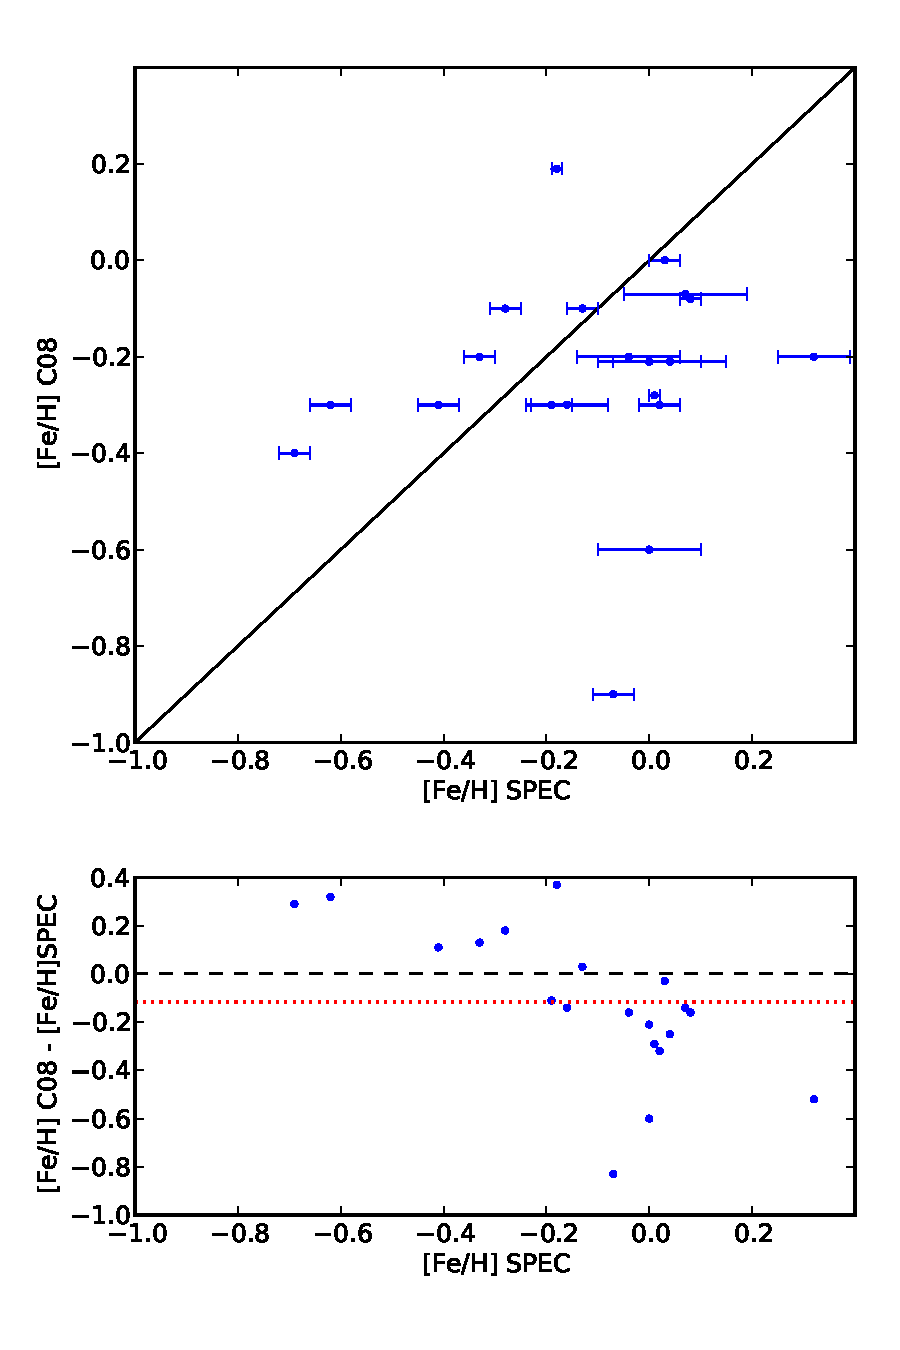
\includegraphics[scale=0.5]{pics/fehfehc08v4.pdf}
\end{center}
\caption{[Fe/H] obtained with the \citet{Casagrande-2008} method versus the spectroscopic metallicity. The blue dots with error bars represent the data points. The black line depicts a one to one relationship. The metallicity difference between the values of the calibrations and the spectroscopic measurements is shown below each [Fe/H]-[Fe/H] plot. The black dashed line is the zero point of the difference, and the red dotted line represents the average of the metallicity difference.  }
\label{fehfehc08}
\end{figure}


We could not directly test the \citet{Casagrande-2008} approach, because there is no published calibration available. However, we used the [Fe/H] values provided by Luca Casagrande, and shown in Table\ref{tablefehc08} to test his method. Following Fig. \ref{fehfehc08} and Table \ref{tablec08}, we can observe that the \citet{Casagrande-2008} method has a higher rms, RMS$_{p}$ and R$^{2}_{ap}$ values when compared to the tested calibrations. The negative R$^{2}_{ap}$ value means that this model is increasing the variance when compared to a constant model. 


\subsection{Calibration of \citet{Rojas-Ayala-2010}}
\label{rojas}

\citet{Rojas-Ayala-2010} recently released a new paper describing a novel and very precise technique that allows an easier observation of M dwarfs. Their technique is based on the calculation of spectral indices via direct spectral analysis of moderate ($R \sim 2700$) near infrared spectra (K band), and has the advantage of not depending on V magnitudes nor parallaxes, allowing the study of fainter (or/and farther) stars. They analysed 17 M dwarfs secondaries with a FGK primary, that served also as metallicity calibrators, and measured the equivalent widths of the NaI doublet (2.206 and 2.209 $\mu m$), and the CaI triplet (2.261, 2.263 and 2.265 $\mu m$). With these measurements and a water absorption spectral index sensitive to stellar temperatures, they constructed a metallicity scale with an adjusted multiple correlation coefficient greater than the one of \citet{Schlaufman-2010} ($R^{2}_{ap} = 0.63$), and also with a tighter RMS$_{p}$ of 0.02 when compared to other studies (0.05, 0.04 and 0.02 for \citet{Bonfils-2005}, \citet{Johnson-2009}, and \citet{Schlaufman-2010} respectively). The metallicity range of the calibration is between -0.5 and +0.5 dex, with an estimated uncertainty of $\pm$0.15 dex.

%Their results agree in general with \citet{Johnson-2009} and \citet{Schlaufman-2010} that M dwarf planet hosts appear to be systematically metal rich, a result consistent with the [Fe/H] distribution of FGK stars with planets. Neptunian host stars also seem to follow the trend of FGK stars, having a lower metallicity than Jovian hosts. \textcolor{green}{Should I erase this paragraph???}

It would be very interesting to test the \citet{Rojas-Ayala-2010} calibration. Unfortunately, we were not able to do it because we lack the infrared spectra to measure the spectral indexes necessary for the calibration. We were able to do an external test, by comparing the measurements of the seven stars in common (Gl 212, Gl 231.1B, Gl 250B, Gl 324B, Gl611B, Gl783.2B, and Gl 797B with predicted [Fe/H] of 0.09, -0.05, -0.04, 0.30, -0.49, -0.19, and -0.06 dex respectively). 
We got a value of only 0.08 dex for the dispersion and a 0.04 dex offset between the spectroscopic measurements and \citet{Rojas-Ayala-2010} predicted metallicities. These numbers have little significance, but they may give a hint that the calibration is compatible with the spectroscopic measurements. With this external test, we cannot confirm or deny if this calibration is better than the one of \citet{Schlaufman-2010}. However, the results suggests that this calibration should be properly tested in the future.


%\subsection{Sample Table}


\begin{sidewaystable*}[]
\tiny
\caption[]{ \label{estrelas}Sample of wide binaries with a FGK primary and a M dwarf secondary. The first and third columns display, respectively, the primary and the secondary stars, along with their respective spectral type (columns two and four). The fifth column depicts the parallaxes of the primary with its associated errors. From the sixth to the twelveth column, the V(RI)$_{C}$JHK$_{S}$ photometry is shown, as well as its associated errors. In the last column, the sources for the photometry are exhibited.}
\begin{tabular}{l c l c r r r r r r r r c}

  \hline
  \hline
Primary&Sp. Type. & Secondary& Sp. Type  &$\pi$&V&R&I&J&H&K$_{s}$&V/RI/JHK source \\
            & primary               &                  &  secondary   & [mas] & [mag] & [mag] & [mag]�& [mag] &�[mag] & [mag] & &  \\

Gl53.1A  &  K4  &  Gl53.1B  &  M3  &  48.20 $\pm$ 1.06  &  13.60 $\pm$ 0.02  &  12.48 $\pm$ 0.05  &  11.01 $\pm$ 0.05  &  9.533 $\pm$ 0.039  &  8.927 $\pm$ 0.023  &  8.673 $\pm$ 0.024  &  W93 / W93 / 2MASS \\
Gl56.3A  &  K1  &  Gl56.3B  &  K7  &  37.75 $\pm$ 0.95  &  10.70 $\pm$ 0.02  &  09.84 $\pm$ 0.03  &  9.01 $\pm$ 0.03  &  8.012 $\pm$ 0.021  &  7.369 $\pm$ 0.029  &  7.190 $\pm$ 0.020  &  B90 / B90 / 2MASS \\
Gl81.1A  &  G9  &  Gl81.1B  &  K7  &  30.44 $\pm$ 0.60  &  11.20 $\pm$ 0.01  &  10.30 $\pm$ 0.01  &  9.41 $\pm$ 0.01  &  8.413 $\pm$ 0.023  &  7.763 $\pm$ 0.021  &  7.597 $\pm$ 0.027  &  C84 / C84 / 2MASS \\
Gl100A  &  K4.5  &  Gl100C  &  M2.5  &  51.16 $\pm$ 1.33  &  12.85 $\pm$ 0.01  &  11.79 $\pm$ 0.01  &  10.43 $\pm$ 0.01  &  9.181 $\pm$ 0.027  &  8.571 $\pm$ 0.029  &  8.347 $\pm$ 0.021  &  C84 / C84 / 2MASS \\
Gl105A  &  K3  &  Gl105B  &  M4  &  139.27 $\pm$ 0.45  &  11.66 $\pm$ 0.02  &  10.45 $\pm$ 0.05  &  8.87 $\pm$ 0.05  &  7.333 $\pm$ 0.018  &  6.793 $\pm$ 0.038  &  6.574 $\pm$ 0.020  &  W93 / W93 / 2MASS \\
Gl140.1A  &  K3.5  &  Gl140.1B  &  K8  &  51.95 $\pm$ 1.16  &  10.17 $\pm$ 0.01  &  - $\pm$ -  &  - $\pm$ -  &  7.436 $\pm$ 0.023  &  6.828 $\pm$ 0.023  &  6.620 $\pm$ 0.040  &  S96 / - / 2MASS \\
Gl157A  &  K4  &  Gl157B  &  M2  &  64.40 $\pm$ 1.06  &  11.61 $\pm$ 0.03  &  - $\pm$ -  &  - $\pm$ -  &  7.773 $\pm$ 0.024  &  7.162 $\pm$ 0.033  &  6.927 $\pm$ 0.031  &  U74 / - / 2MASS \\
Gl173.1A  &  K3  &  Gl173.1B  &  M3  &  32.69 $\pm$ 1.51  &  14.19 $\pm$ 0.02  &  13.05 $\pm$ 0.05  &  11.65 $\pm$ 0.05  &  10.263 $\pm$ 0.022  &  9.715 $\pm$ 0.028  &  9.421 $\pm$ 0.024  &  W93 / W93 / 2MASS \\
Gl211  &  K1  &  Gl212  &  M0  &  81.44 $\pm$ 0.54  &  09.76 $\pm$ 0.01  &  8.81 $\pm$ 0.05  &  7.76 $\pm$ 0.05  &  6.586 $\pm$ 0.021  &  5.963 $\pm$ 0.016  &  5.759 $\pm$ 0.016  &  HIP / W93 / 2MASS \\
Gl231.1A  &  G0  &  Gl231.1B  &  M3.5  &  51.95 $\pm$ 0.40  &  13.27 $\pm$ 0.02  &  12.15 $\pm$ 0.05  &  10.62 $\pm$ 0.05  &  9.088 $\pm$ 0.023  &  8.559 $\pm$ 0.042  &  8.267 $\pm$ 0.018  &  WT81 / WT81 / 2MASS \\
Gl250A  &  K3  &  Gl250B  &  M2  &  114.94 $\pm$ 0.86  &  10.08 $\pm$ 0.01  &  09.04 $\pm$ 0.01  &  7.80 $\pm$ 0.01  &  6.579 $\pm$ 0.034  &  5.976 $\pm$ 0.055  &  5.723 $\pm$ 0.036  &  L89 / L89 / 2MASS \\
Gl297.2A  &  F6.5  &  Gl297.2B  &  M2  &  44.68 $\pm$ 0.30  &  11.80 $\pm$ 0.02  &  - $\pm$ -  &  - $\pm$ -  &  8.276 $\pm$ 0.019  &  7.672 $\pm$ 0.027  &  7.418 $\pm$ 0.016  &  R04 / - / 2MASS \\
Gl324A  &  G8  &  Gl324B  &  M4  &  81.03 $\pm$ 0.75  &  13.16 $\pm$ 0.01  &  11.94 $\pm$ 0.05  &  10.27 $\pm$ 0.05  &  8.560 $\pm$ 0.027  &  7.933 $\pm$ 0.040  &  7.666 $\pm$ 0.023  &  D88 / WT77 / 2MASS \\
Gl559A  &  G2  &  Gl551  &  M6  &  772.33 $\pm$ 2.42  &  11.05 $\pm$ 0.02  &  9.43 $\pm$ 0.03  &  7.43 $\pm$ 0.03  &  5.357 $\pm$ 0.023  &  4.835 $\pm$ 0.057  &  4.31 $\pm$ 0.03  &  B90 / B90 / 2MASS \\
Gl611A  &  G8  &  Gl611B  &  M4  &  68.87 $\pm$ 0.33  &  14.23 $\pm$ 0.02  &  13.00 $\pm$ 0.05  &  11.38 $\pm$ 0.05  &  9.903 $\pm$ 0.021  &  9.453 $\pm$ 0.021  &  9.159 $\pm$ 0.017  &  W96 / W96 / 2MASS \\
Gl653  &  K5  &  Gl654  &  M2  &  93.40 $\pm$ 0.94  &  10.07 $\pm$ 0.01  &  9.10 $\pm$ 0.01  &  7.95 $\pm$ 0.01  &  6.780 $\pm$ 0.029  &  6.193 $\pm$ 0.021  &  5.975 $\pm$ 0.026  &  K02 / K02 / 2MASS \\
Gl666A  &  G8  &  Gl666B  &  M0  &  113.61 $\pm$ 0.69  &  08.70 $\pm$ 0.01  &  - $\pm$ -  &  - $\pm$ -  &  7.237 $\pm$ 9.999  &  5.112 $\pm$ 0.023  &  4.856 $\pm$ 0.020  &  E79 / - / 2MASS \\
Gl783.2A  &  K1  &  Gl783.2B  &  M4  &  49.04 $\pm$ 0.65  &  14.06 $\pm$ 0.02  &  12.81 $\pm$ 0.03  &  11.20 $\pm$ 0.03  &  9.627 $\pm$ 0.018  &  9.108 $\pm$ 0.015  &  8.883 $\pm$ 0.018  &  DS92 / DS92 / 2MASS \\
Gl797A  &  G5  &  Gl797B  &  M2.5  &  47.65 $\pm$ 0.76  &  11.87 $\pm$ 0.01  &  - $\pm$ -  &  - $\pm$ -  &  8.160 $\pm$ 0.020  &  7.645 $\pm$ 0.023  &  7.416 $\pm$ 0.016  &  D82 / - / 2MASS \\
GJ3091A  &  K2  &  GJ3092B  &  M  &  33.83 $\pm$ 1.00  &  15.64 $\pm$ 0.03  &  13.81 $\pm$ 0.05  &  11.97 $\pm$ 0.05  &  11.092 $\pm$ 0.023  &  10.540 $\pm$ 0.026  &  10.266 $\pm$ 0.021  &  P82 / E76 / 2MASS \\
GJ3194A  &  G4  &  GJ3195B  &  M3  &  41.27 $\pm$ 0.58  &  12.55 $\pm$ 0.02  &  11.49 $\pm$ 0.05  &  10.15 $\pm$ 0.05  &  8.877 $\pm$ 0.021  &  8.328 $\pm$ 0.023  &  8.103 $\pm$ 0.029  &  W96 / W96 / 2MASS \\
GJ3627A  &  G5  &  GJ3628B  &  M3.5  &  38.58 $\pm$ 2.17  &  14.10 $\pm$ 0.03  &  12.88 $\pm$ 0.05  &  11.31 $\pm$ 0.05  &  9.828 $\pm$ 0.022  &  9.247 $\pm$ 0.021  &  9.015 $\pm$ 0.018  &  W88 / W88 / 2MASS \\
NLTT34353  &  G5  &  NLTT34357  &  K7  &  20.73 $\pm$ 1.05  &  12.41 $\pm$ 0.02  &  11.51 $\pm$ 0.03  &  10.59 $\pm$ 0.03  &  9.595 $\pm$ 0.026  &  8.910 $\pm$ 0.026  &  8.734 $\pm$ 0.019  &  R89 / R89 / 2MASS \\

\hline
\end{tabular}

References. [W93] \citet{Weis-1993}; [B90] \citet{Bessell-1990}; [C84] \citet{Caldwell-1984}; [S96] \citet{Sinachopoulos-1996}; [U74] \citet{Upgren-1974}; [HIP] \citet{ESA-1997}; [W81] \citet{Weistrop-1981}; [L89] \citet{Laing-1989}; [R04] \citet{Reid-2004}; [D88] \citet{Dahn-1988};  [W77] \citet{Weistrop-1977}; [W96] \citet{Weis-1996}; [K02] \citet{Koen-2002}; [E79] - \citet{Eggen-1979} [D92] - \citet{Dawson-1992}; [D82] \citet{Dahn-1982}; [P82] \citet{Pesch-1982}; [E76] \citet{Eggen-1976}; [W88] \citet{Weis-1988}; [R89] \citet{Ryan-1989}; [B91] \citet{Bessell-1991}; [2MASS] \citet{Skrutskie-2006}.
\end{sidewaystable*}



\end{document}




%\begin{table}[b]
%\caption{Stellar parameters for \object{HD\,45652}.}
%\label{table:hd45652_star}
%\begin{tabular}{lcc}
%\hline\hline
%\noalign{\smallskip}
%Parameter  & Value & Reference \\
%\hline
%Spectral~type                   & K5/G8-K0              & Hipparcos/This Paper \\
%$m_v$                           & 8.1                   & Hipparcos \\
%$B-V$                           & 0.85                  & Hipparcos \\
%Distance~[pc]                   & 36$\pm$2              & Hipparcos \\
%$v~\sin{i}$~[km~s$^{-1}$]       & $<$2$\dagger$  	& This paper \\
%$\log{R'_\mathrm{HK}}$	        & $-$4.90$\pm$0.10$\dagger\dagger$      & This paper \\
%$T_{\rm eff}$~[K]               & 5312$~\pm~$68         & This paper \\
%$\log{g}$~[cgi]                 & 4.32$~\pm~$0.21       & This paper \\
%$\xi_{\mathrm{t}}$              & 0.89$~\pm~$0.09       & This paper \\
%${\rm [Fe/H]}$                  & $+$0.29$~\pm~$0.07    & This paper \\
%Mass~$[M_{\odot}]$              & 0.83$\pm$0.05         & This paper \\
%\hline
%\noalign{\smallskip}
%\end{tabular}
%\newline
%$\dagger$ From ELODIE spectra using a calibration similar to the one presented by \citet{Santos-2002a}\\
%$\dagger\dagger$ From SOPHIE spectra using a calibration similar to the one presented by \citet{Santos-2000a}
%\end{table}
%
%
%\begin{figure}[t]
%\resizebox{\hsize}{!}{\includegraphics{09402F2.eps}}
%\caption{{\it Top}: ELODIE (red circles), CORALIE (blue squares), and SOPHIE (magenta diamonds) 
%radial-velocities for HD\,45652 as a function of time, and the best Keplerian fit to the 
%data. {\it Bottom}: residuals of the fit.} 
%\label{fig:time}
%\end{figure}
%
%